%%%%%%%%%%%%%%%%%%%%%%%%%%%%%%%%%%%%%%%%%%%%%%%%%%%%%%%
%                 File: OSAtemp.tex                   %
%                Date: Sept. 2. 2009                  %
%                                                     %
%    LaTeX template file for use with OSA journals    %
%         JOSA A, JOSA B, and Applied Optics          %
%
%                                                     %
%   This file requires the substyle file osajnl2.rtx, %
%       running under REVTeX 4.0 and LaTeX 2e,        %
%                           or                        %
%   the style file osajnl2.sty, running under LaTeX 2e%
%                                                     %
%       USE THE FOLLOWING REVTEX 4.0 OPTIONS:         %
%  \documentclass[osajnl2,preprint,showpacs]{revtex4} %
%                                                     %
%         USE THE FOLLOWING LaTeX OPTIONS:            %
%           \documentclass[12pt]{article}             %
%           \usepackage{osajnl2}                      %
%                                                     %
%                                                     %
%      (C) 2009 The Optical Society of America        %
%                                                     %
%%%%%%%%%%%%%%%%%%%%%%%%%%%%%%%%%%%%%%%%%%%%%%%%%%%%%%%

%\documentclass[12pt,osajnl2,preprint,showpacs]{revtex4}  %% REVTeX 4.0

%%%%%%%%%%%%%%%%%%%%%%%%%%%%%%%%%%%%%%%%%%%%%%%%%%%%%%%%%%%%%%%%
%% Delete any REVTEX output files before running in LaTeX mode
%%%%%%%%%%%%%%%%%%%%%%%%%%%%%%%%%%%%%%%%%%%%%%%%%%%%%%%%%%%%%%%%%

\documentclass[letterpaper,12pt]{article}   %% LaTeX 2e (preferred)
\usepackage{osajnl2} %% do not use with REVTeX4
\usepackage[draft,implicit=false]{hyperref} %% optional
\usepackage{caption}
\usepackage{subcaption}
\usepackage{algcompatible}
\usepackage{algorithm}
%\usepackage{algorithmic}
\usepackage{chngpage}
\usepackage{geometry}
\usepackage{wrapfig}

%This then gives you access to:
%\begin{wrapfigure}[lineheight]{position}{width}

%****************************************************************************
% Shireen Elhabian formating additions

\newenvironment{myindentpar}[1]%
     {\begin{list}{}%
             {\setlength{\leftmargin}{#1}\setlength{\rightmargin}{#1}}%
             \item[]%
     }
     {\end{list}}
     

\setlength{\parskip}{0pt}
\setlength{\parsep}{0pt}
\setlength{\headsep}{0pt}
\setlength{\topskip}{0pt}
\setlength{\topmargin}{0pt}
\setlength{\topsep}{0pt}
\setlength{\partopsep}{0pt}
\setlength{\itemsep}{0pt}
\setlength{\textfloatsep}{0.1in}%{-0.2in}
\setlength{\intextsep}{0pt}
\setlength{\dblfloatsep}{0.05in}
\setlength{\dbltextfloatsep}{0.1in}
\setlength{\belowcaptionskip}{0in}
\setlength{\abovecaptionskip}{0in}
%\setlength{\bibsep}{0.0pt}
\setlength{\belowdisplayskip}{0pt} \setlength{\belowdisplayshortskip}{0pt}
\setlength{\abovedisplayskip}{0pt} \setlength{\abovedisplayshortskip}{0pt}


%****************************************************************************
\usepackage{amsmath}
\usepackage{listings}
%\newcommand{\argmin}{\operatornamewithlimits{argmin}}
%\newcommand{\argmax}{\operatornamewithlimits{argmax}}

\DeclareMathOperator*{\argmax}{arg\!\max}

%% to have figures at the top of the page
%\makeatletter
%\setlength{\@fptop}{0pt}
%\makeatother

\lstdefinestyle{BashInputStyle}{
  language=bash,
  basicstyle=\small\ttfamily,
  %numbers=left,
  numberstyle=\tiny,
  numbersep=3pt,
  %frame=tb,
  framerule=1pt,
  %columns=fullflexible
  frame=single,
  breaklines=true,
  postbreak=\raisebox{0ex}[0ex][0ex]{\ensuremath{\color{red}\hookrightarrow\space}}
}

\usepackage{wrapfig}
\graphicspath{{figures/}}
\begin{document}

\title{ShapeWorksStudio Lab Walkthrough}
\begin{figure}
\centering

\includegraphics[scale=1]{figs/shapes-icon.png}
\end{figure}

%% For REVTeX it is possible to automate superscript and e-mail callouts with the superscriptaddress option; see REVTeX4 documentation.


\author{ShapeWorks Team}
\vspace{0.1in}
\email{shapeworks-users@sci.utah.edu}
\vspace{0.2in}
\address{School of Computing, University of Utah, Salt Lake City, UT 84112, USA}

\vspace{0.5in}

\hrule
\tableofcontents
\vspace{0.02in}
\hrule
%\newpage

\section{Requirements}

\begin{itemize}
    \item Git \texttt{(https://git-scm.com/)}
    \item CMake 2.6+ \texttt{(http://www.cmake.org/)}
    \item Visualization ToolKit (VTK 6+ recommended) \texttt{(http://www.vtk.org/)}
    \item Insight Toolkit (ITK 4.5+ recommended) \texttt{(http://www.itk.org/)}
    \item Qt 4.8.* \texttt{(http://www.qt.io/developers/)}
    \item Windows 7+, OSX 10.7+, and OpenSuse 13.1 Recommended. Other platforms may work, but are not officially supported.
    \item Shapeworks command line tools (Groom and Run) are required for Studio \texttt{(https://github.com/SCIInstitute/shapeworks/releases)}
\end{itemize}

\section{Building}

\subsection{Unix and OSX}

In a terminal:

\begin{lstlisting}[style=BashInputStyle]
mkdir ShapeWorksStudio/build
cd ShapeWorksStudio/build
cmake -DVTK_DIR=Path/To/Your/VTK/build -DITK_DIR=Path/To/Your/ITK/build -DShapeworksCLT_BINARY_DIR=Path/To/ShapeWorks/Binaries -DCMAKE_BUILD_TYPE=Release ../src
make
\end{lstlisting}


\subsection{Windows}

Open a Visual Studio (32 or 64 bit) Native Tools Command Prompt. Follow these commands:

\begin{lstlisting}[style=BashInputStyle]
mkdir C:\Path\To\ShapeWorksStudio\build
cd C:\Path\To\ShapeWorksStudio\build
cmake -G "NMake Makefiles" -DVTK_DIR="C:/Path/To/Your/VTK/build" -DITK_DIR="C:/Path/To/Your/ITK/build" -DShapeworksCLT_BINARY_DIR="C:/Path/To/ShapeWorks/Binaries" -DCMAKE_BUILD_TYPE=Release ../src
nmake
\end{lstlisting}

NOTE: Be sure to copy the Qt DLL files to the Executable directory for the program to run.

\section{Running}

Studio runs with no command-line arguments. Double click the generated binary file in Windows/Mac or use \texttt{./ShapeWorksStudio} on Linux terminal.  You should have a Qt window that looks similar to the one shown in Fig. \ref{fig:qtwin}. The application has tools on the left, the rendering window, view options on the lower bar, a small file menu, and a preferences dialog.

\begin{figure}[!htp]
\centering
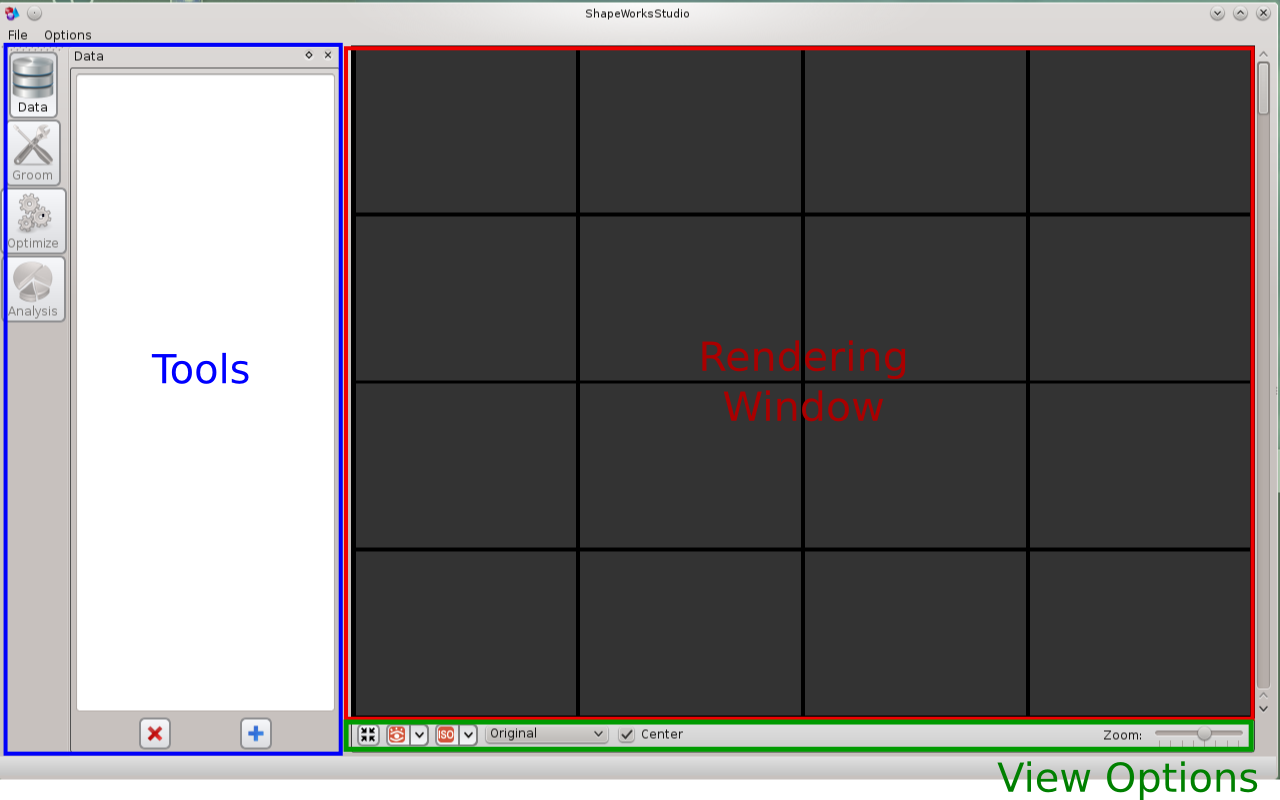
\includegraphics[width=0.9\textwidth]{figs/qtwin2.png}
\caption{Initial ShapeWorksStudio window}
\label{fig:qtwin}
\end{figure}

\section{Tools}

\subsection{Data}

This tool tab displays the images (volume files in NRRD format) that have been loaded. You can select the image files to load by either clicking the blue "+" button at the bottom (see Fig. \ref{fig:add}), or going to \texttt{File -> Import Images} (see Fig. \ref{fig:import}). Once the file import dialog appears, you can select multiple files to be loaded to your studio project (see Fig. \ref{fig:torusfiles}). Your images will appear on the display once loaded (see Fig. \ref{fig:torusimages}). You can delete images by selecting the image of choice and clicking the red "x" button at the bottom (see Fig. \ref{fig:remove}). 

It is recommended to continuously save your project by pressing \texttt{Ctrl+S} or using the file menu (see Fig. \ref{fig:save}) in order to be able to resume your project after closing the current session. Studio is smart enough to ask you to save your project upon leaving (see Fig. \ref{fig:close}). Studio project file is an xml file containing the list of images being imported to your project and the corresponding files generated from different stages (i.e. grooming, optimization and analysis).

\begin{figure}[!htp]
\centering

\includegraphics[width=0.9\textwidth]{figs/add.png}
\caption{Import binary volumes using the blue "+" button}
\label{fig:add}
\end{figure}

\begin{figure}[!htp]
\centering
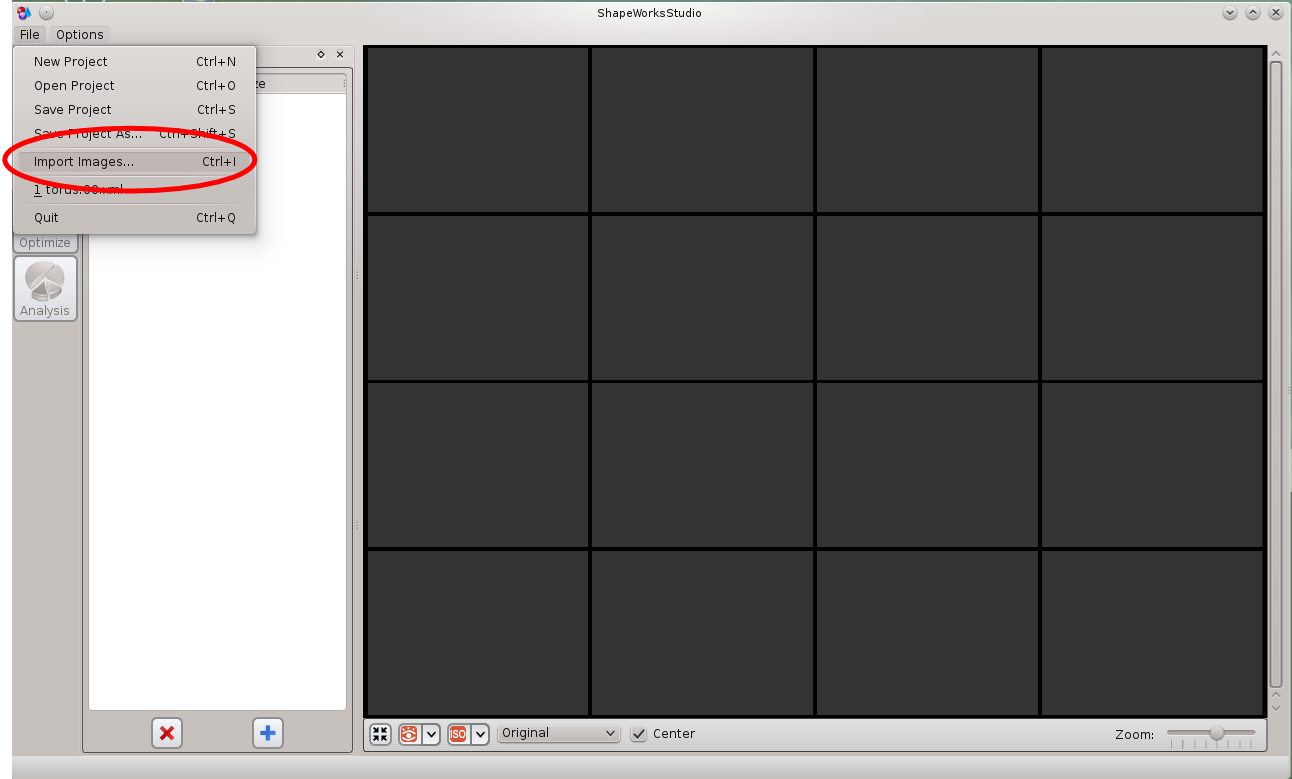
\includegraphics[width=0.9\textwidth]{figs/import.png}
\caption{Import binary volumes from the file menu}
\label{fig:import}
\end{figure}

\begin{figure}[!htp]
\centering
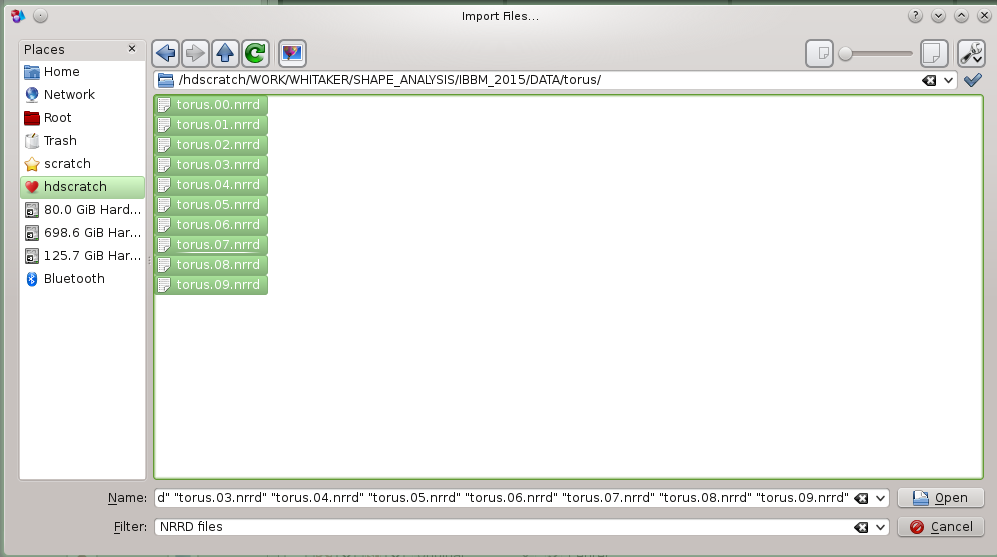
\includegraphics[width=0.9\textwidth]{figs/torusfiles.png}
\caption{Selection of multiple files to be loaded to your studio project}
\label{fig:torusfiles}
\end{figure}

\begin{figure}[!htp]
\centering
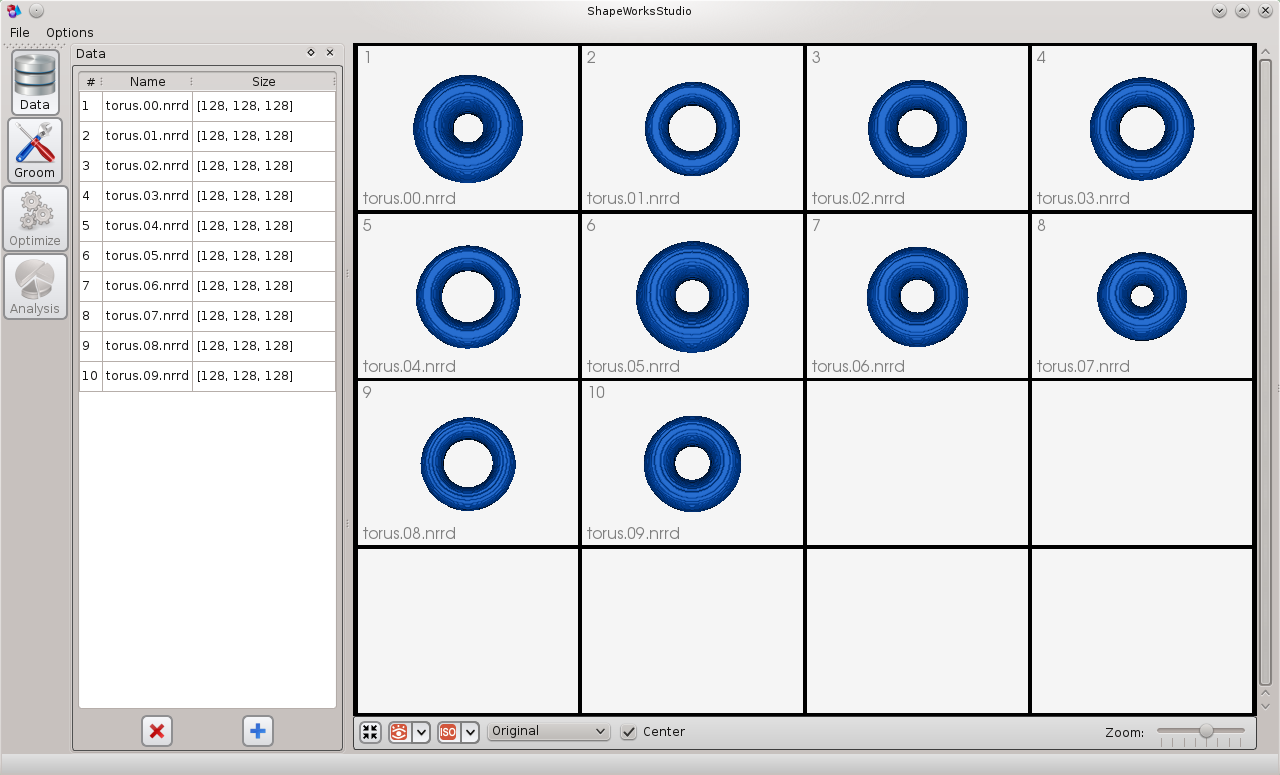
\includegraphics[width=0.9\textwidth]{figs/torusimages.png}
\caption{After loading the images: Left: the \texttt{Data} panel shows the files names and the image sizes. Right: the rendering window displays the isosurface of the binary images that have been loaded to your project}
\label{fig:torusimages}
\end{figure}

\begin{figure}[!htp]
\centering
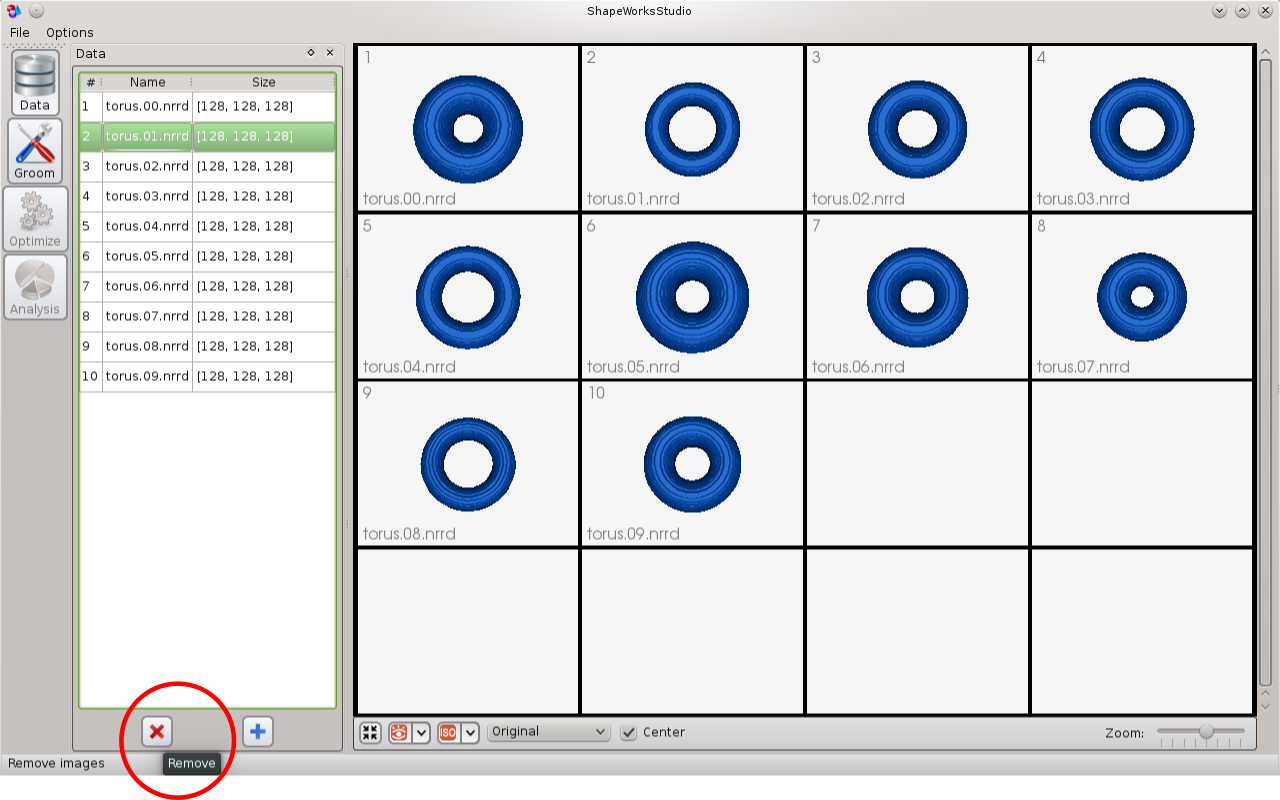
\includegraphics[width=0.9\textwidth]{figs/remove.png}
\caption{At any time, you can select an image to be removed from your project using the red "x" button}
\label{fig:remove}
\end{figure}

\begin{figure}[!htp]
\centering
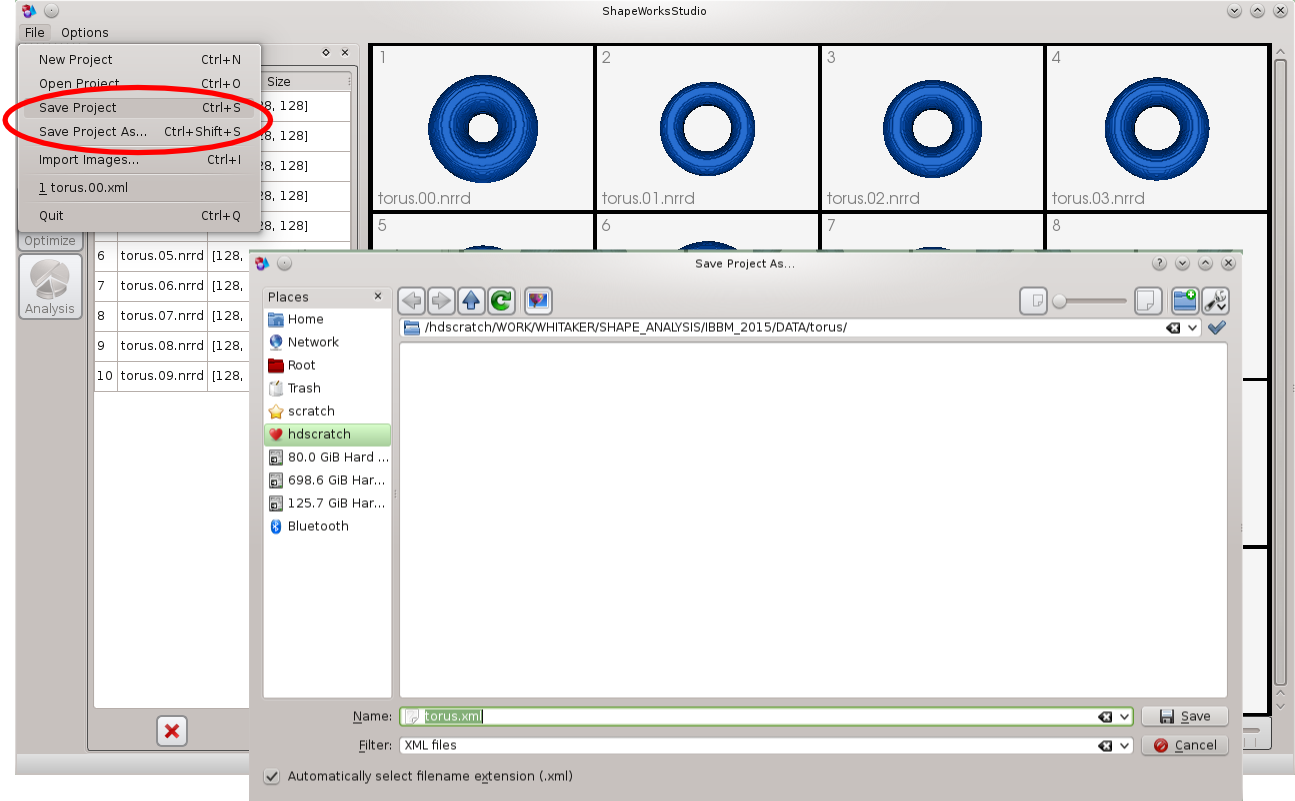
\includegraphics[width=0.9\textwidth]{figs/save.png}
\caption{Saving your project}
\label{fig:save}
\end{figure}

\begin{figure}[!htp]
\centering
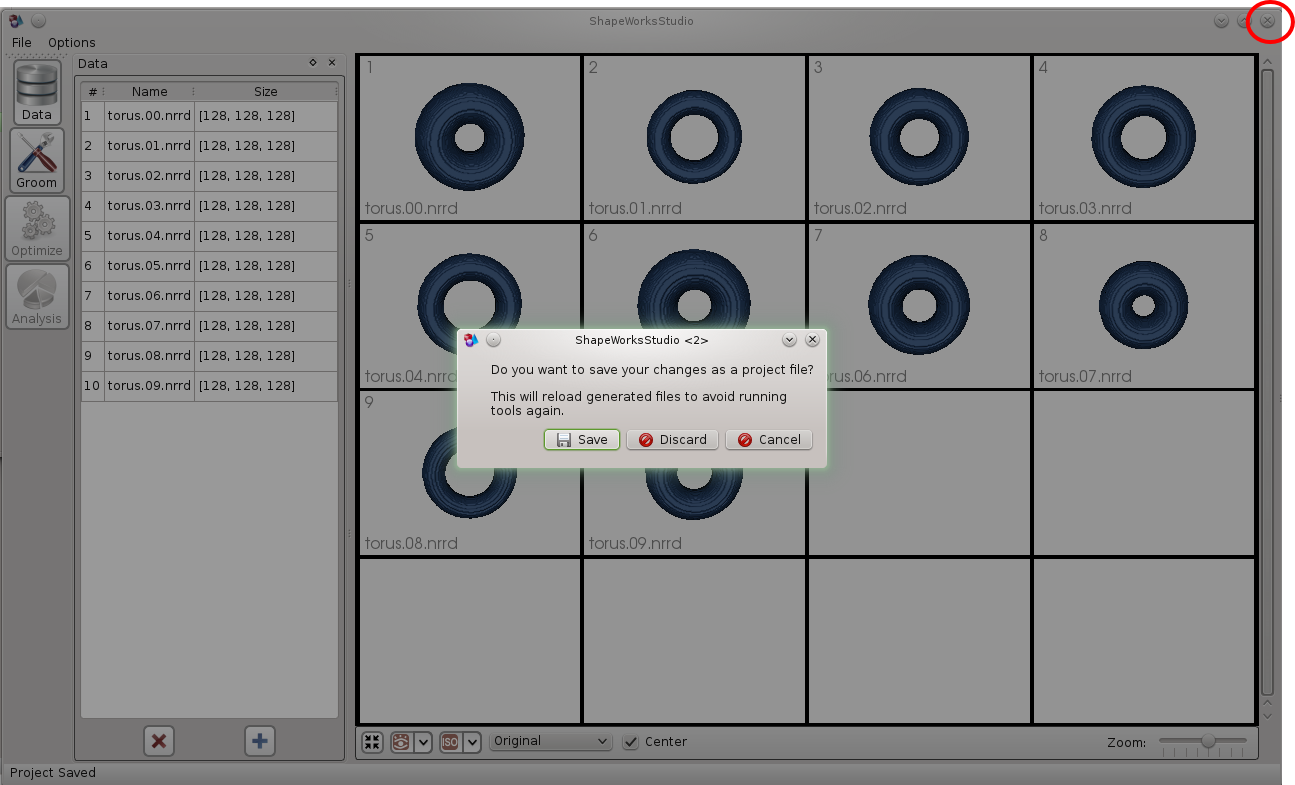
\includegraphics[width=0.9\textwidth]{figs/close.png}
\caption{Studio asks you to save your project upon closing}
\label{fig:close}
\end{figure}

\subsection{Groom}

Once images are loaded, the preprocessing step, \textit{"groom"} is next. You can select several options for grooming (see Fig. \ref{fig:groom}).

\begin{itemize}
\item \textbf{Fill Holes:} This option fills any existing holes in the loaded segmentations.

\item \textbf{Isolate:} This option isolates the foreground (non-zero voxels) from the background.

\item \textbf{Center:} This option attempts to align the segmentations to a common center if they aren't sharing the same center

\item \textbf{Autocrop:} Use this option to find the largest bounding box containing all input shapes, and crop all input volumes accordingly.

\item \textbf{Pad:} This option adds a padding around the shapes. This is helpful when the segmentations are very close to or touching the volume boundaries. Padding the volumes would help the optimization step to keep the particles within the volume boundaries without shooting the particles outside, especially at high curvature regions. The selected padding amount is the number of voxels to be padded in each dimension.

\item \textbf{Antialias:} This option antialiases the binary segmentation in order to remove the staircase effect at shapes' isosurfaces resulting from the abrupt change of a binary image between a background and a foreground voxel. The resulting antialiased volumes will have a smooth transition between foreground and background regions. You can select the number of antialias iterations with more iterations resulting in a smoother transition.

\item \textbf{Fastmarching:} This option computes a signed distance transform of the surface using the Fast Marching method.

\item \textbf{Blur:} This option blurs the resulting distance transforms to get rid of high-frequency artifacts. You can choose an appropriate sigma for the blurring with higher sigma values resulting in smoother surfaces. Sigma values are relative to the images spacing. It is recommended not to use high values of sigma that would error thin structures in your shapes.

\item \textbf{Run Groom:} Click this when you are ready for grooming. This step takes some time. You can monitor the output messages on the terminal or refer to ShapeWorksStudioTools.log file next to the executable. A progress tasks indicator shows the tool is working. In case you are not satisfied with the groomed shapes, e.g. too smooth, you can always modify any of the aforementioned parameters and click "Run Groom".

\item \textbf{Export XML:} If you wish to use the parameter file created for the groom step in a command line environment, you can export the XML with the grooming options above.

\end{itemize}

Fig. \ref{fig:groomed} shows the resulting groomed shapes for a torus ensemble. Note that you can use the drop-down menu from the viewing options bar at the bottom to switch between the original and the groomed shapes. You can also use the \texttt{Zoom} slide bar to display less or more shapes in the rendering window grid and thus see more or less details for individual shapes (see Fig. \ref{fig:zoom}).

\vspace{0.05in}
\begin{figure}[!htp]
  \begin{minipage}[c]{0.7\textwidth}
  \centering
    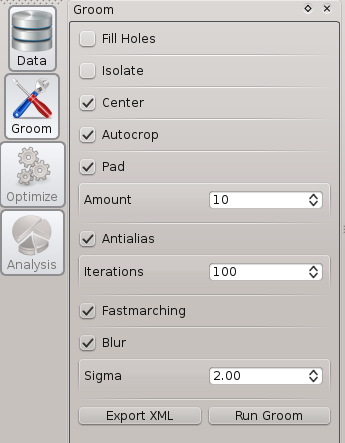
\includegraphics[width=0.6\textwidth]{figs/groom.png}
  \end{minipage}\hfill
  \begin{minipage}[c]{0.3\textwidth}
  \centering
    \caption{\texttt{Groom}-ing your shapes is a preprocessing step that would convert the input binary images to their corresponding implicit representation for ShapeWorks while taking care of aliasing artifacts} 
    \label{fig:groom}
  \end{minipage}
\end{figure}

\begin{figure}[!htp]
\centering
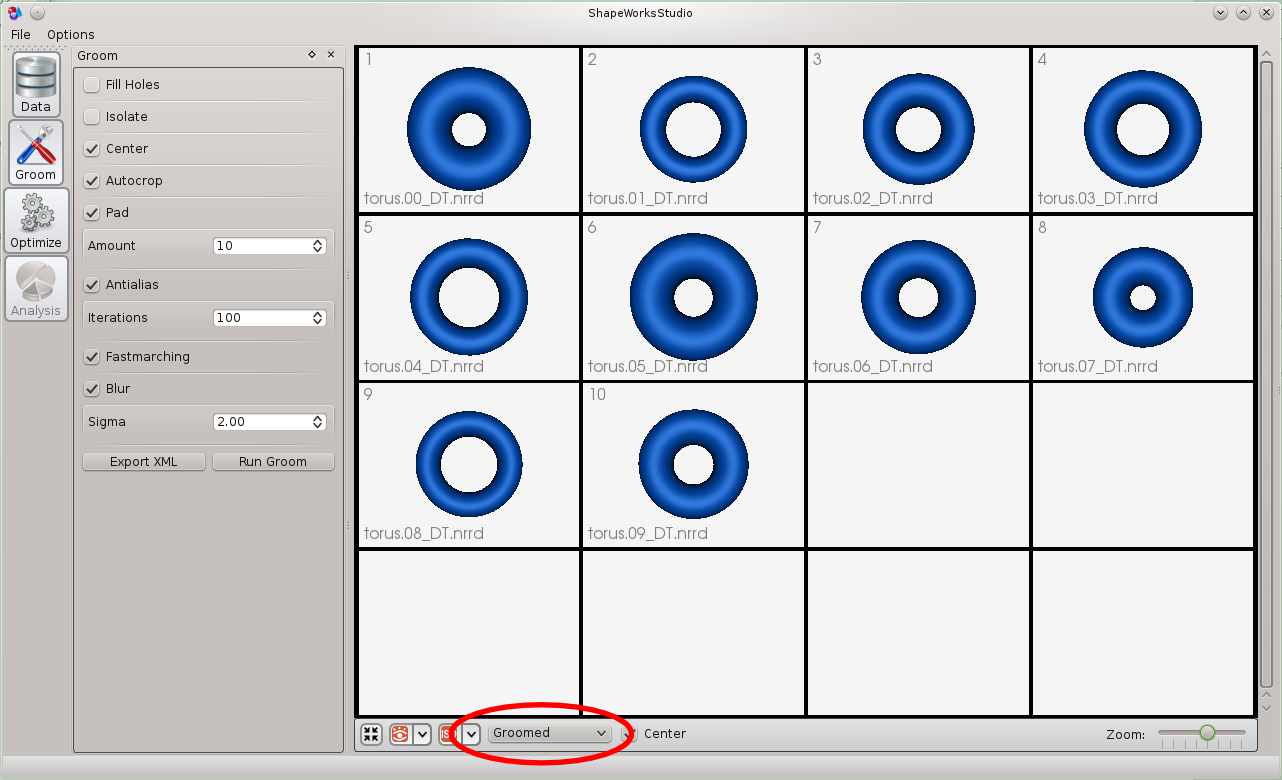
\includegraphics[width=0.9\textwidth]{figs/groomed.png}
\caption{Groomed shapes, refer to the viewing options to switch between original and groomed shapes}
\label{fig:groomed}
\end{figure}

\begin{figure}[!htp]
\centering
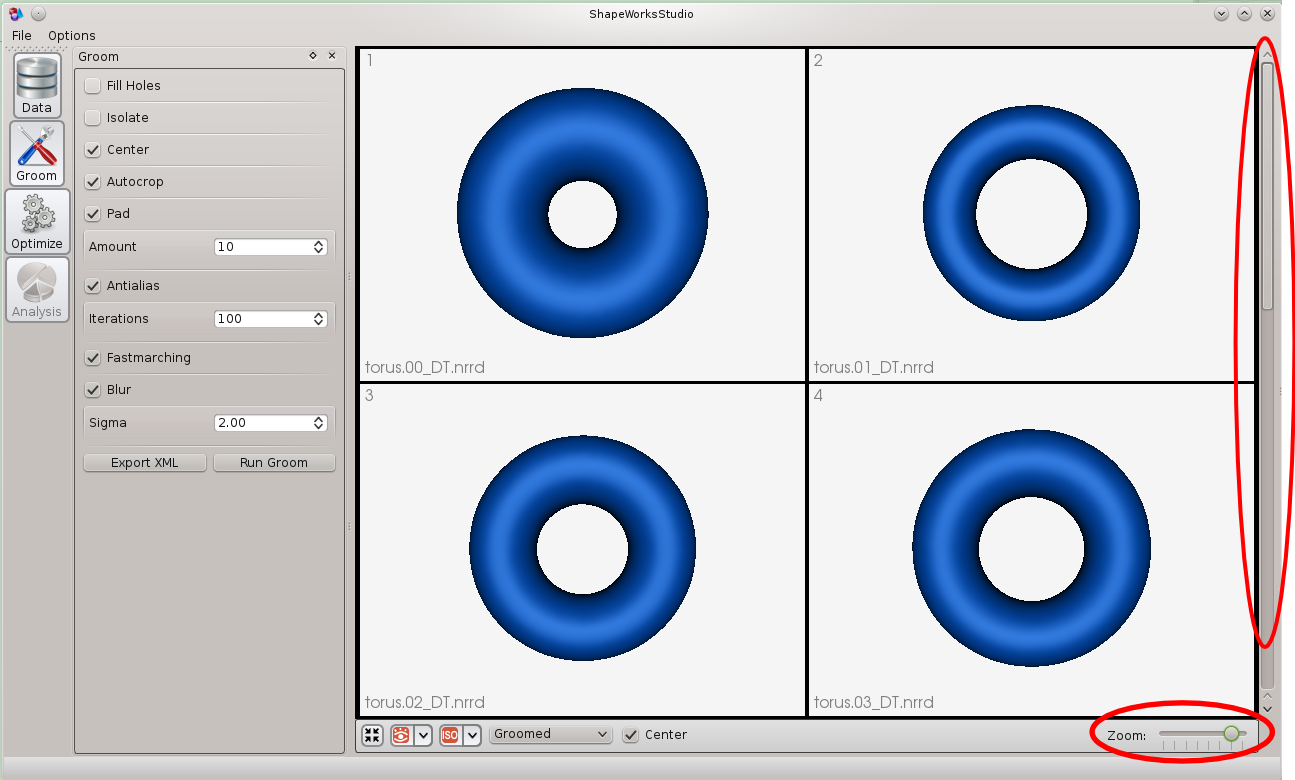
\includegraphics[width=0.9\textwidth]{figs/zoom.png}
\caption{Use the \texttt{Zoom} slide bar to zoom in/out to display less or more number of shapes. Use the slide bar to move down/up in case of showing a small number of shapes}
\label{fig:zoom}
\end{figure}

\subsection{Optimize}

Once the grooming step is complete, you can run the optimize step which involves uniformly spreading corresponding particles over the isosurfaces of the groomed shapes. You can control the optimization process via tuning the following parameters (see Fig. \ref{fig:optimize}):

\begin{itemize}
\item \textbf{Number of points:} Specifies the number of particles to be used to represent each shape in the ensemble with more particles enables capturing geometrical shape details. %If enough initial particle positions are supplied for the optimization, then the commandline tool \texttt{ShapeWorksRun} will not conduct a splitting-based initialization phase. If insufficient particle initializations are supplied (or none at all), then \texttt{ShapeWorksRun} will initialize the model as described in Section 2.3 until this number of particles exists on each shape surface.

\item \textbf{Starting/Ending Regularization:} This option determines the regularizations on the covariance matrix for the shape-space entropy estimation. This regularization exponentially decay along optimization iterations where better covariance structure can be estimated with better correspondence model. Higher regularization values would undermine the underlying covariance structure of the ensemble. Hence it is recommended to use starting regularization value as $\approx 5\%$ of the expected highest eigenvalue of the covariance matrix while ending regularization can be taken as ten times less than the starting value. 

\item \textbf{Iterations per split:} Specifies the number of iterations to run between successive particle splits during an initialization phase. This allows the particle system at a given granularity to converge to a stable state before more particles are added.

\item \textbf{Optimization Iterations:} Specifies the number of optimization iterations to be performed in order to yield optimized correspondence model. %Specify the range for a constant regularization factor that is added to the covariance matrix of the correspondences during the optimization process. This range, along with the number of optimization iterations, define the rate at which the system converges. The starting regularization decays to the ending regularization over the specified number of iterations.

\item \textbf{Relative Weighting:} This is the value of parameter "alpha" from the energy equation $Q = H(Z) - \alpha * \sum_k H(x_k)$. This parameters weights the sampling part of the objective function with lower values give more important to the correspondence entropy and higher values guides the optimization towards better surface sampling. Recommended value is $1$, yet for some ensembles, one might tune this parameter to balance the trade-off between surface sampling and particle correspondence. Figs. \ref{fig:rel1} and \ref{fig:rel100} show the optimized correspondence models using 1 and 100 as relative weighting values, respectively. Figs \ref{fig:rel1_hover1}-\ref{fig:rel100_hover2} show visual correspondence inspection where it can be observed that when using higher relative weighting, i.e. allowing surface sampling to dominate the optimization process, resulting particles become out-of-correspondence.

\item \textbf{Run Optimize:} Click this when you are ready for optimizing. This step takes time, but relatively less than grooming. However, the timing depends primarily on number of shapes, number of particles and number of iterations specified. You can watch the terminal to keep track of intermediate output which is also written to ShapeWorksStudioTools.log file next to the executable. A progress indicator shows the tool is working. Upon completion, the rendering working will show the optimized correspondence model, i.e. particles, overlayed onto their particle-based reconstructed surfaces.

\item \textbf{Export XML:} If you wish to use the parameter file created for the groom step in a command line environment, you can export the XML with the grooming options above. There are other options not in the GUI that you can add to a parameter file to run outside of Studio.
\end{itemize}

\vspace{0.05in}
\begin{figure}[!htp]
  \begin{minipage}[c]{0.7\textwidth}
  \centering
    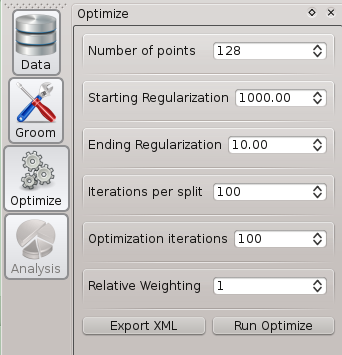
\includegraphics[width=0.6\textwidth]{figs/optimize.png}
  \end{minipage}\hfill
  \begin{minipage}[c]{0.3\textwidth}
  \centering
    \caption{\texttt{Optimize} involves uniformly spreading corresponding particles over the isosurfaces of the groomed shapes. You can control this process by setting the parameters shown } 
    \label{fig:optimize}
  \end{minipage}
\end{figure}
\vspace{0.1in}
\begin{figure}[!htp]
\centering
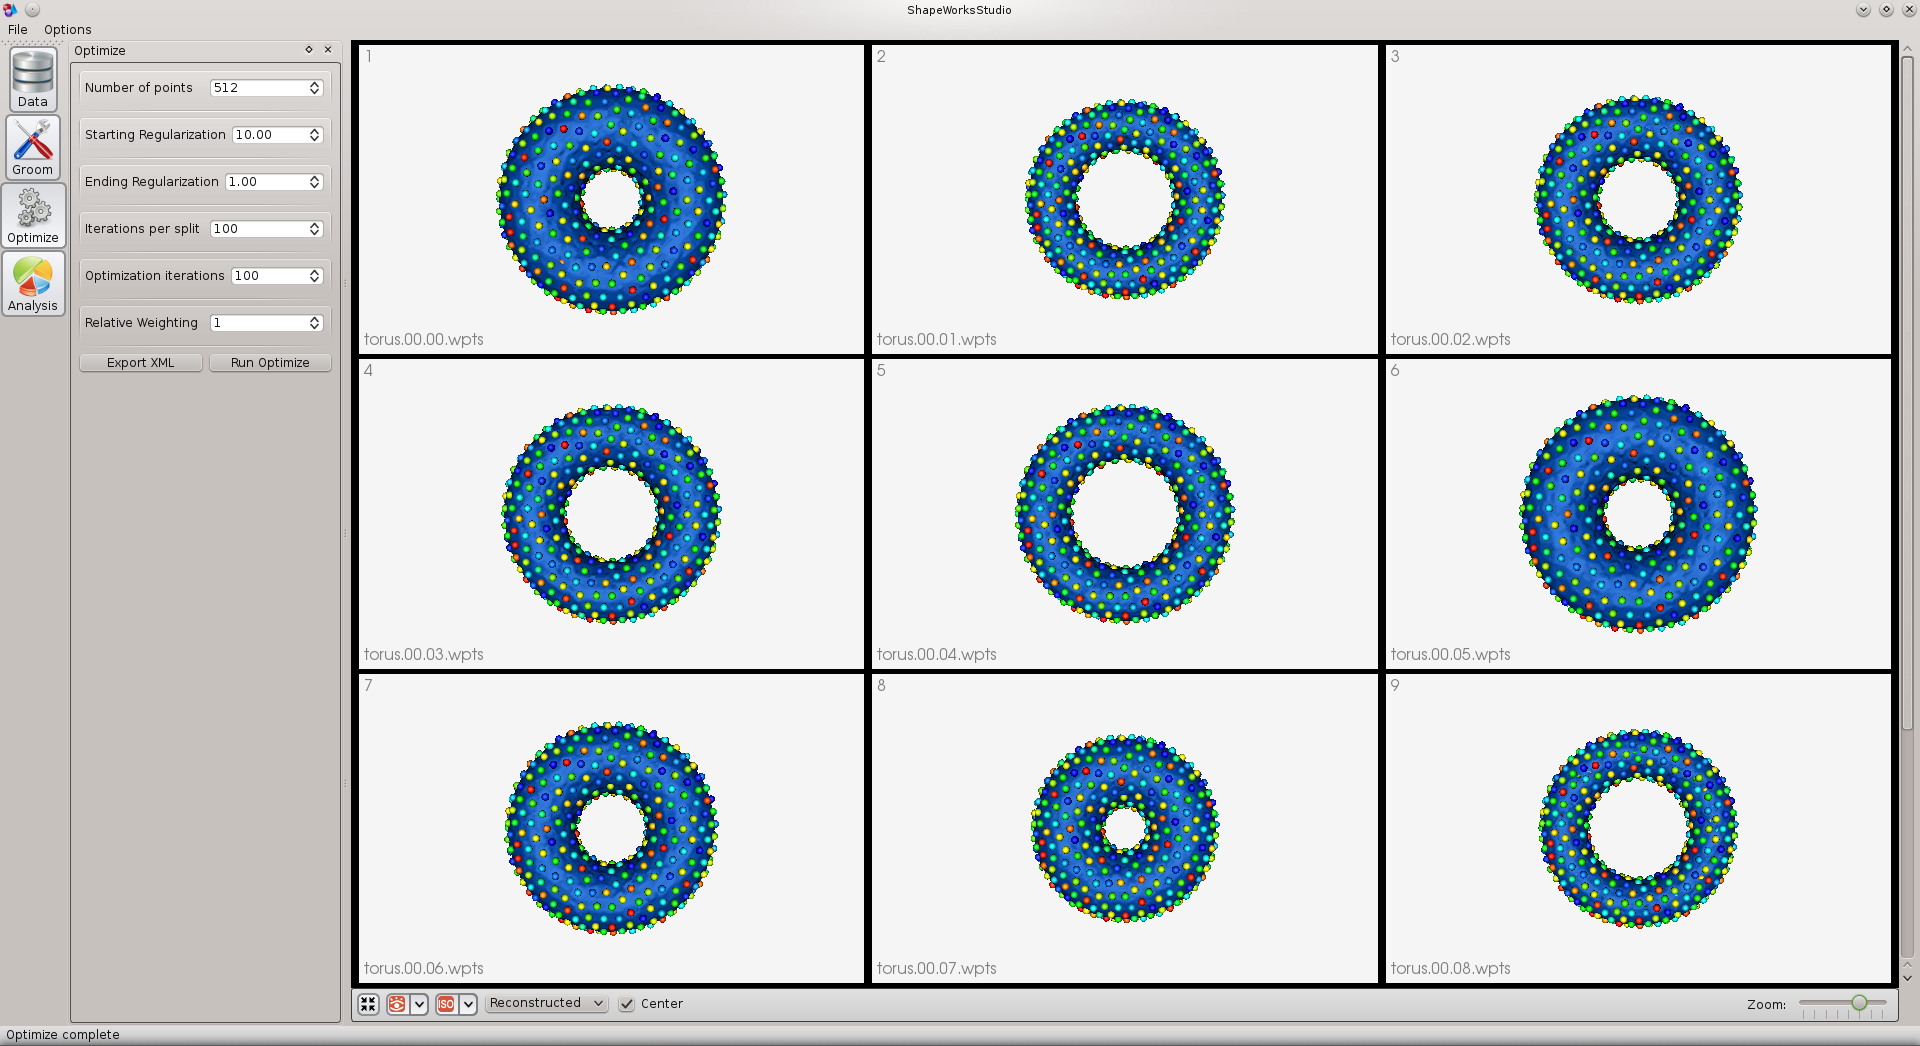
\includegraphics[width=0.9\textwidth]{figs/relative_1.png}
\caption{Optimized correspondence model using relative weighting $ = 1$}
\label{fig:rel1}
\end{figure}

\begin{figure}[!htp]
\centering
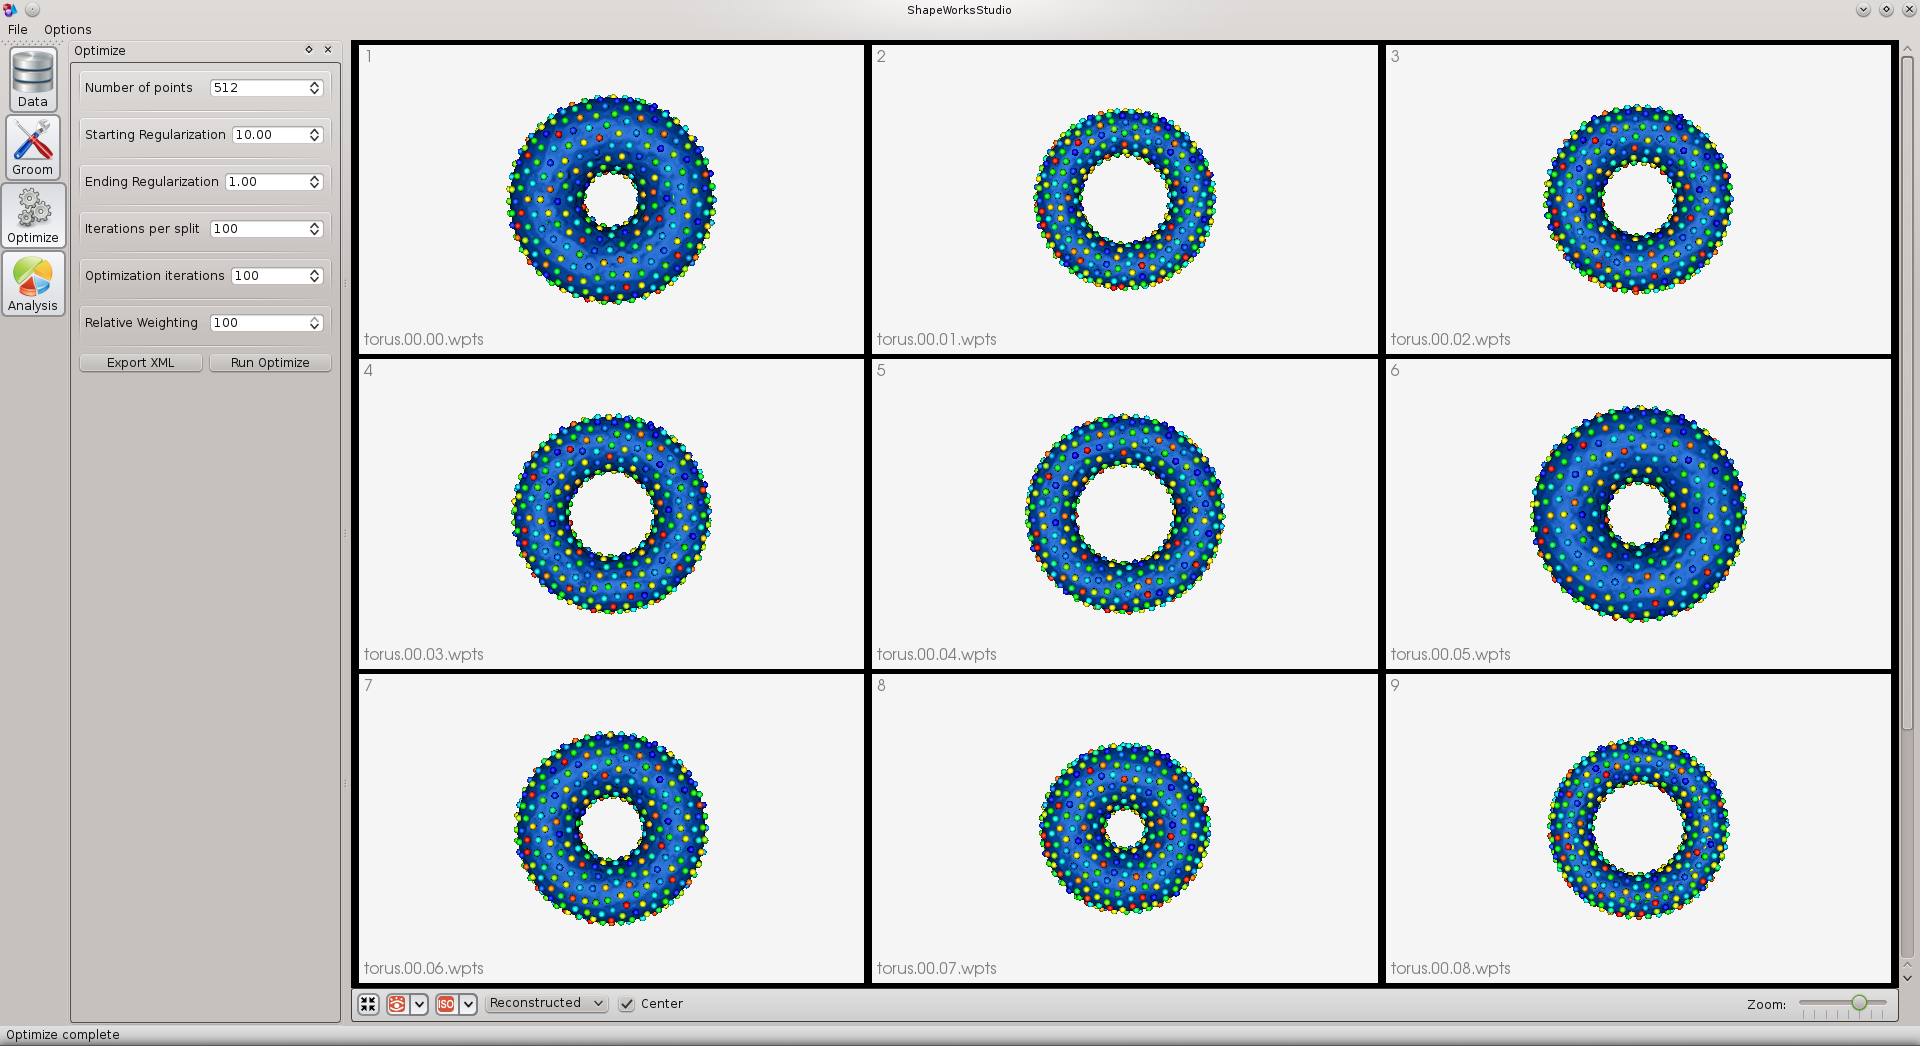
\includegraphics[width=0.9\textwidth]{figs/relative_100.png}
\caption{Optimized correspondence model using relative weighting $ = 100$}
\label{fig:rel100}
\end{figure}

\begin{figure}[!htp]
\centering
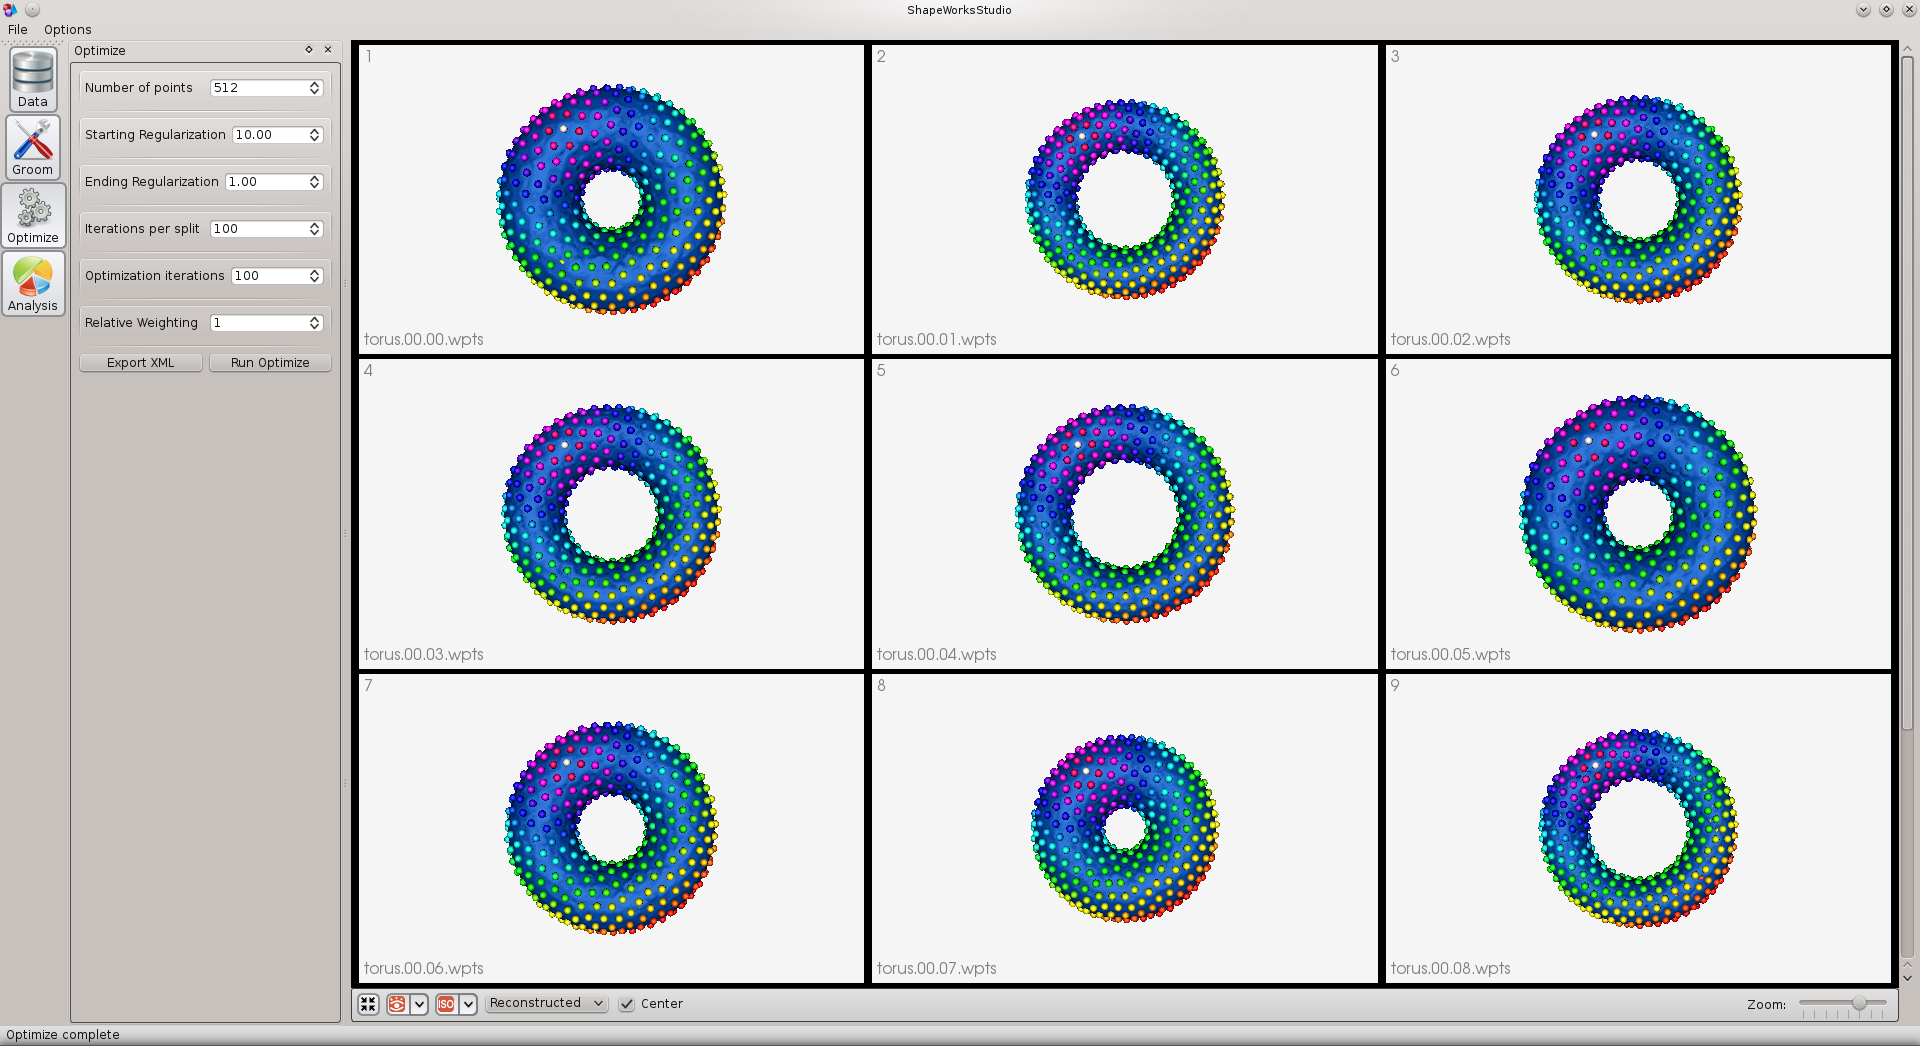
\includegraphics[width=0.9\textwidth]{figs/rel1_hover1.png}
\caption{Optimized correspondence model using relative weighting $ = 1$ with one particle selected to visualize correspondence. Simply hover on the required particle and press 1, the particle will be colored in white and all other particles will be colored based on its distance to the selected particle. To recover the original display, type 1 or 2 while NOT hovering over any particles}
\label{fig:rel1_hover1}
\end{figure}

\begin{figure}[!htp]
\centering
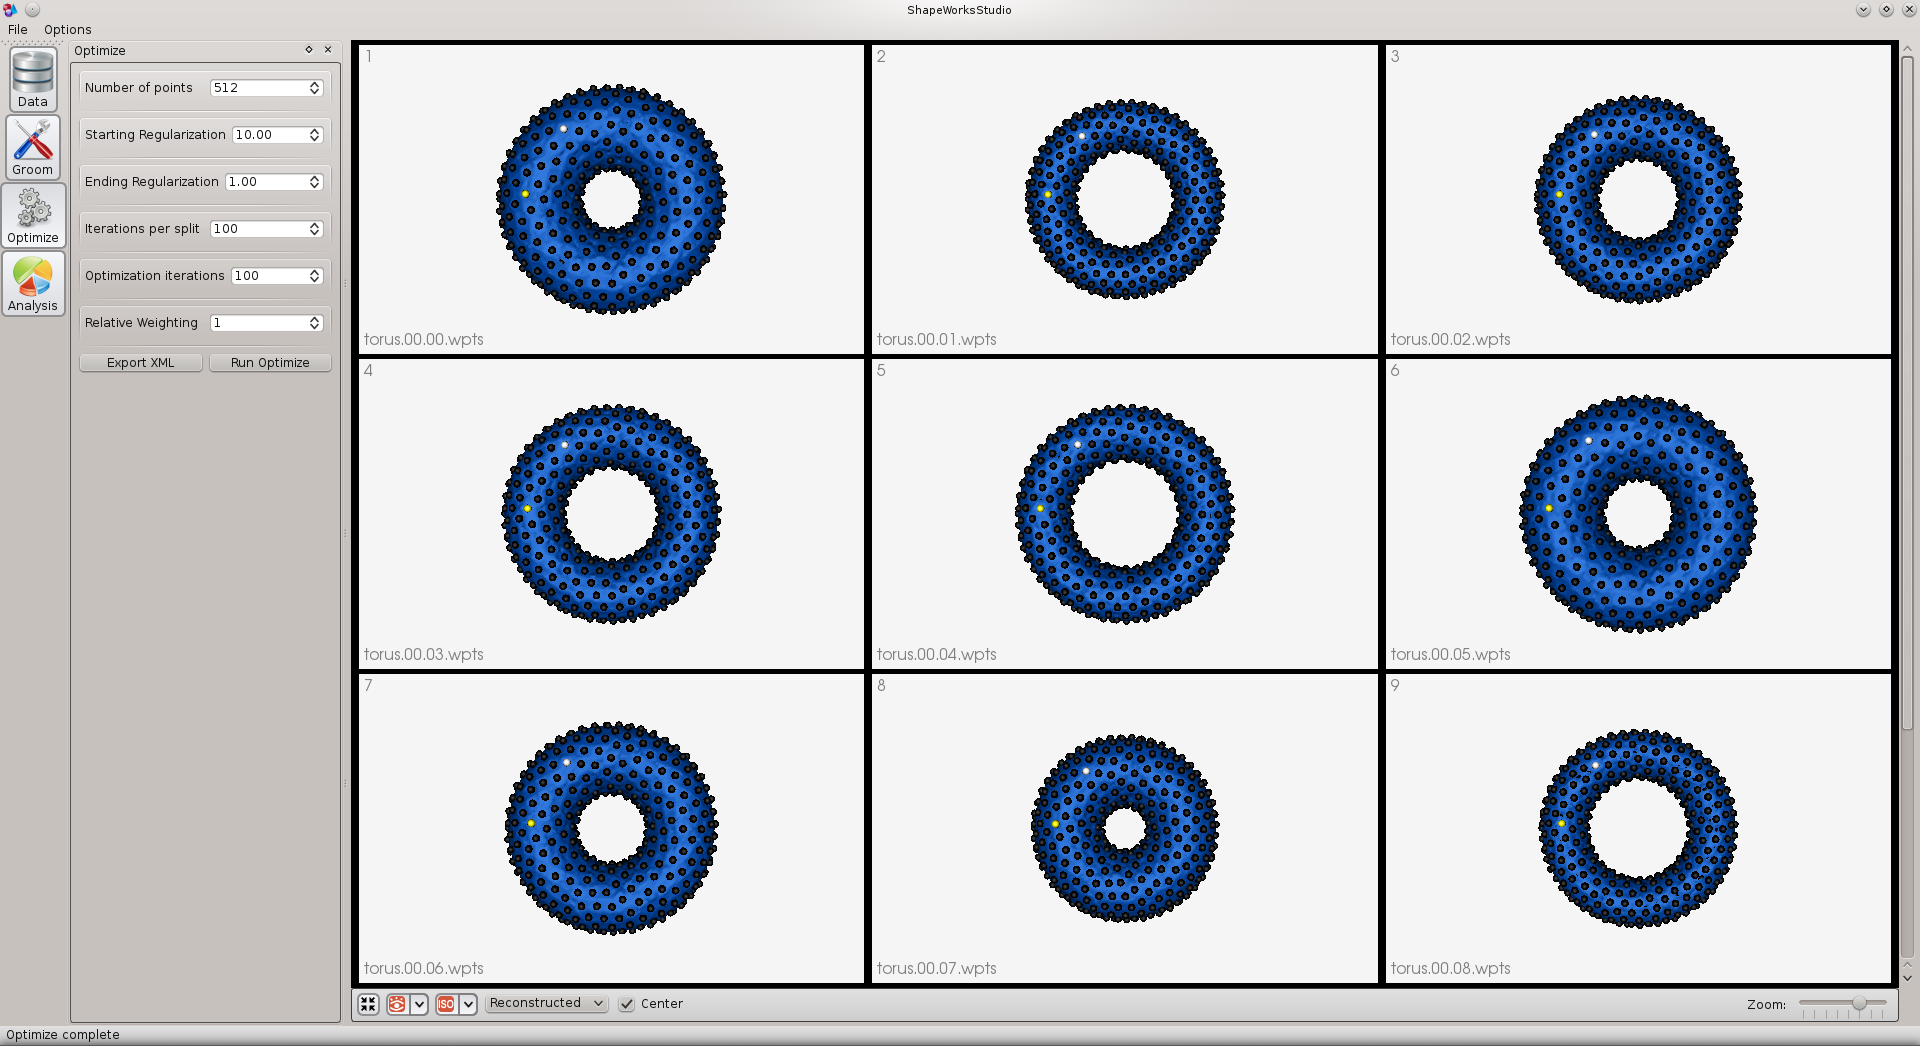
\includegraphics[width=0.9\textwidth]{figs/rel1_hover2.png}
\caption{Optimized correspondence model using relative weighting $ = 1$ with two particles selected to visualize pairwise correspondence. Simply hover on the second required particle and press 2, the second particle will be colored in yellow and all other particles will be colored in black. To recover the original display, type 1 or 2 while NOT hovering over any particles}
\label{fig:rel1_hover2}
\end{figure}


\begin{figure}[!htp]
\centering
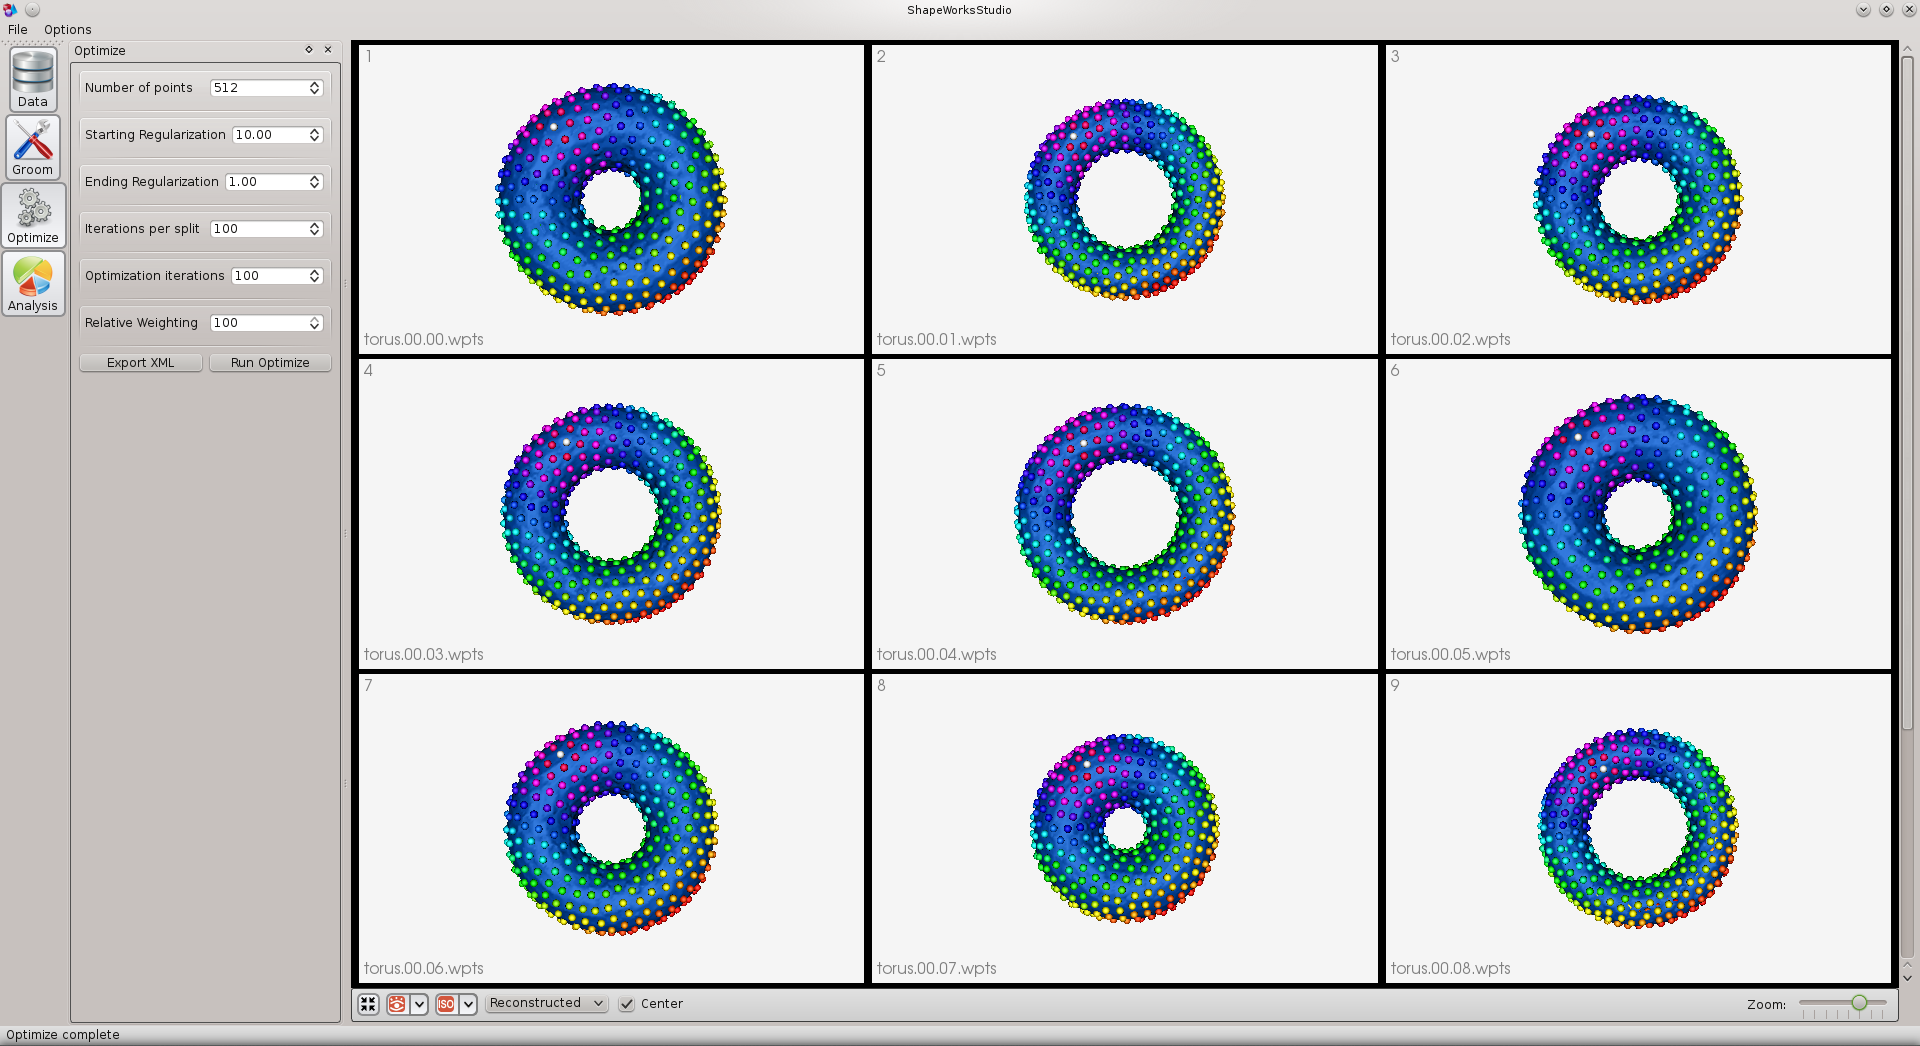
\includegraphics[width=0.9\textwidth]{figs/rel100_hover1.png}
\caption{Optimized correspondence model using relative weighting $ = 100$ with one particle selected to visualize correspondence. Simply hover on the required particle and press 1, the particle will be colored in white and all other particles will be colored based on its distance to the selected particle. . To recover the original display, type 1 or 2 while NOT hovering over any particles. Note that particles are out-of-correspondence since surface sampling is dominating the optimization process}
\label{fig:rel100_hover1}
\end{figure}

\begin{figure}[!htp]
\centering
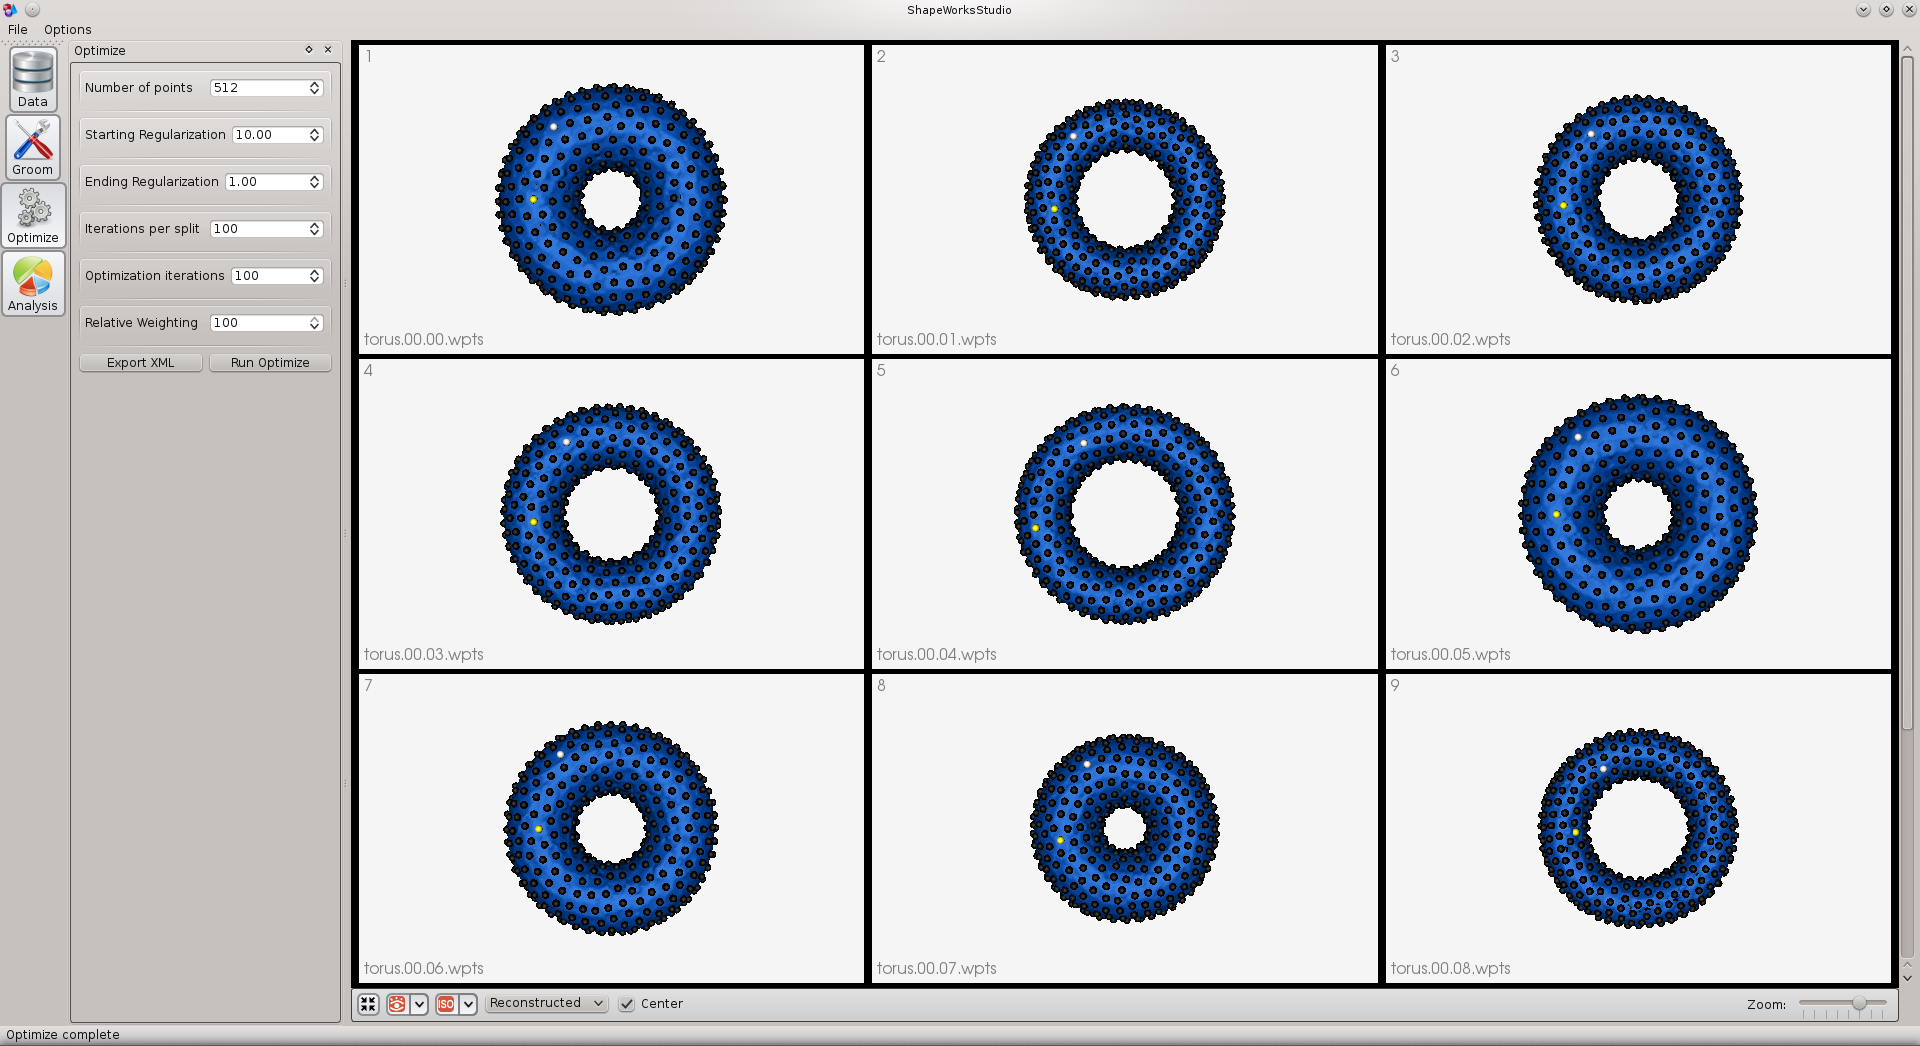
\includegraphics[width=0.9\textwidth]{figs/rel100_hover2.png}
\caption{Optimized correspondence model using relative weighting $ = 100$ with two particles selected to visualize pairwise correspondence. Simply hover on the second required particle and press 2, the second particle will be colored in yellow and all other particles will be colored in black. . To recover the original display, type 1 or 2 while NOT hovering over any particles. Note that particles are out-of-correspondence since surface sampling is dominating the optimization process}
\label{fig:rel100_hover2}
\end{figure}

\subsection{Analysis}

\begingroup
\setlength\intextsep{0pt}

\begin{wrapfigure}{r}{0.43\textwidth}
  \centering
    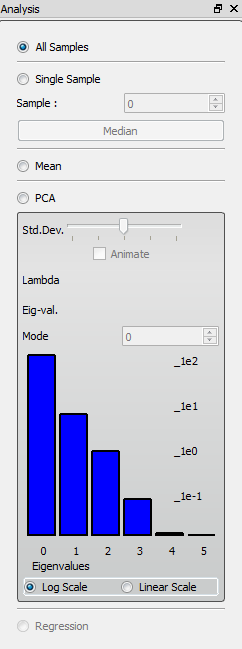
\includegraphics[width=0.43\textwidth]{figs/analysis.png}
  \caption{Analysis step}
\label{fig:analysis}
\end{wrapfigure}

The analysis step is where all the statistical options are available to the user. The following options are available (see Fig. \ref{fig:analysis}):

\begin{itemize}
\item \textbf{All Samples:} Display all of the shape samples along with the correspondence model (i.e. corresponding particles) on the screen.
\item \textbf{Single Sample:} Display only one sample. You can select a particular number, or click "median" to display the shape that is the computed median of all the shapes.
\item \textbf{Mean:} Display the computed mean of the shapes based on the optimized correspondence model.
\item \textbf{PCA:} Display the computed shape from an eigen value and a standard deviation.
\item \textbf{Std.Dev.:} Slide the slider back and forth to display the computed shape with various standard deviations.
\item \textbf{Animate:} Check this box to watch the shape morph between various standard deviations automatically. Depending on the machine running the application, the number of samples, and the size of the samples, the animation may be slow at first while building and caching the meshes. You can select the caching, memory, and threading options in the Preferences. Changing the number of neighbors, spacing, and smoothing options in preferences also affects meshing time and quality.
\end{itemize}

\endgroup

%\begin{wrapfigure}{r}{0.4\textwidth}
%  \centering
%    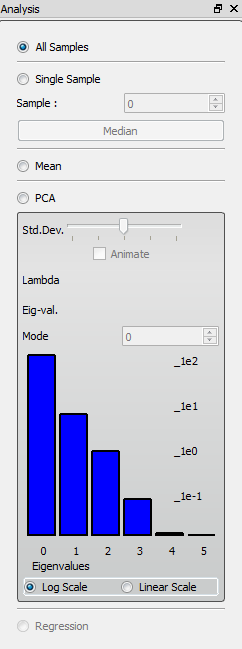
\includegraphics[width=0.4\textwidth]{figs/analysis.png}
%  \caption{Analysis step}
%\label{fig:analysis}
%\end{wrapfigure}

\begin{itemize}
\item \textbf{Mode:} This selects the ordered eigen vector and eigen values from the statistical analysis. There are number of samples - 1 modes. The higher the mode, the less variance with the standard deviations. Usually the first hand full of modes contain the most variance between shapes.

\item \textbf{Log Scale vs. Linear Scale:} The bar graph, displaying the eigen values spectrum of the optimized model, can be plotted in either log or linear scaling. The graph shows the eigen values in decreasing values to depict statistical relevancy. Fig. \ref{fig:specturms} shows the spectrums of the optimized models using relative weight 1 and 100 respectively. 

\item \textbf{Regression:} This option is not yet available.

\end{itemize}


\begin{figure}[!htp]
\centering
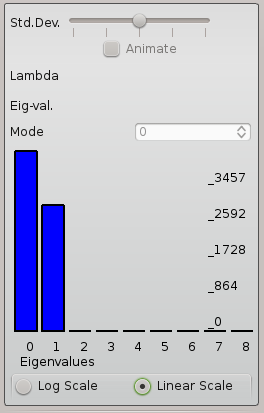
\includegraphics[width=0.4\textwidth]{figs/spectrum_rel1.png}
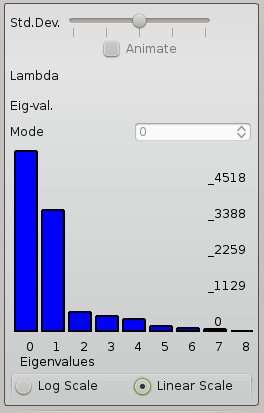
\includegraphics[width=0.4\textwidth]{figs/spectrum_rel100.png}
\caption{Eigenvalue spectrum for correspondence model with relative weighting $= 1$ (left) and $ = 100$ (right). Notice a more compact statistical model (left) is achieved when balancing the trade-off between surface sampling and particle correspondence, reflecting the fact that particles are in better correspondence compared to using high relative weighting for surface sampling }
\label{fig:specturms}
\end{figure}

\section{Rendering Window}

\begin{figure}[!htp]
\centering
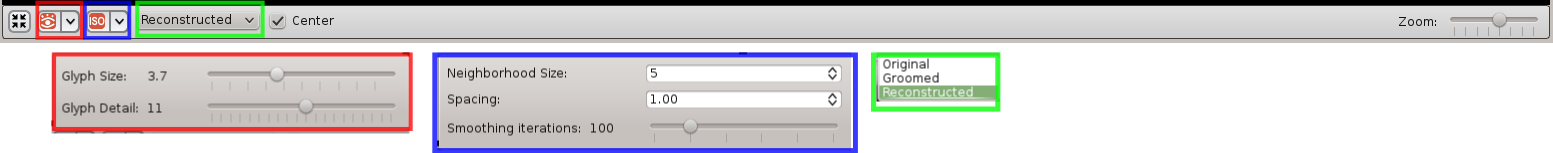
\includegraphics[width=1\textwidth]{figs/render.png}
\caption{Rendering options}
\label{fig:render}
\end{figure}

The render window has a few shortcuts to viewing options (see Fig. \ref{fig:render}). From left to right, here are the rendering options:

\begin{itemize}

\item \textbf{Autoview:} Reset the view to fit the samples. This only affects zoom and translation.

\item \textbf{Show Glyphs:} Toggle whether to show the glyphs for the correspondence points.

\item \textbf{Glyph Quality:} This slider changes the quality of the correspondence points glyphs. This is sync'd with the render window shortcut option.

\item \textbf{Glyph Size:} This slider changes the size of the correspondence points glyphs. This is sync'd with the render window shortcut option.

\item \textbf{Glyph options:} Click the down arrow to resize the glyphs or select the quality of the glyphs.

\item \textbf{Show isosurface:} Toggle whether to view the surface representing the shape. Click the down arrow for more options. You can alter the number of neighbors, point spacing, and mesh smoothing for isosurface reconstruction.

\item \textbf{Neighborhood Size:} The neighborhood size (max vertex valence) used for isosurface reconstruction.

\item \textbf{Spacing:} The spacing used for isosurface reconstruction.

\item \textbf{Smoothing:} The smoothing amount for isosurface reconstruction.

\item \textbf{View mode drop-down:} This drop-down gives 3 options for view mode. Original is the binary segmentation. You must have loaded images for this option to be available. Groomed is for the distance transform view. You must
run the groom step for this to be available. Reconstructed is for the calculated shape based on the set of correspondence points. You must run the optimize step for this to be available.

\item \textbf{Center:} Center the samples automatically to align. This is useful if original samples aren't the same size.

\item \textbf{Zoom:} This slider allows the user to zoom in or out to view more/less samples. This is mainly useful in the "All Samples" mode of the analysis tool. Zoom is automatically selected as a user switches between analysis modes.

\end{itemize}

\begin{figure}[!htp]
\centering
    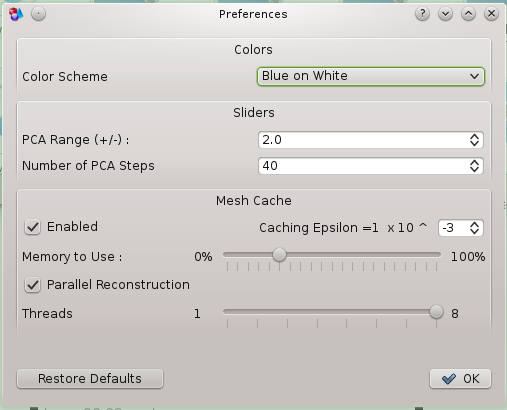
\includegraphics[width=0.5\textwidth]{figs/pref.png}
\caption{Preferences}
\label{fig:pref}
\end{figure}

\section{Preferences}

\begin{itemize}
\item \textbf{Color Scheme:} Select the color scheme for the rendering window.

\item \textbf{PCA Range:} This is the amount of standard deviation to reach on the +/- ends of the PCA Slider.

\item \textbf{Number of PCA Steps:} This determines how many steps between +/- PCA Range to take for visualization.

\item \textbf{Enable Caching:} To speed up mesh animation, you can cache the meshes into system memory to load as needed.

\item \textbf{Caching Epsilon:} How sensitive the caching is. The smaller the epsilon, the more meshes that will be cached, even if they are very similar. If this is too high, large mesh differences might be ignored.

\item \textbf{Memory to Use:} Select the amount of system memory to use for caching. Turn this down if your machine's memory is bogged down from the program.

\item \textbf{Parallel Reconstruction:} Select the amount of threads to fire (up to system hardware core max) to run while building meshes. This speeds reconstruction, theoretically.

\item \textbf{Restore Defaults:} Click this to restore all options to the program's default values. Options are saved and reloaded between application runs for convenience.

\item \textbf{OK:} Click this when you are done changing options.

\end{itemize}


\section{File Menu}

Here you can open and save projects, load new images, open recent projects, and quit the application.
\section{More Examples}

We generated 3 synthetic datasets, each with 30 binary images (133$\times$133$\times$133 voxels) with unit spacing using 3D parametric surfaces named as supershapes with 3 rotational symmetries. Supershapes can be parameterized in polar coordinates as, 
\begin{equation}
	r(\phi) = \left[ \left|\frac{\cos(m\phi/4)}{a} \right|^{n_2} + \left|\frac{\sin(m\phi/4)}{b} \right|^{n_3} \right]^{-1/n_1},
\end{equation}
where we set $m = 3$ (rotational symmetries), $a = b = 1$ and $n_1 = 4$. 

In order to mimic one mode of shape variation, The dataset \texttt{supershape3\char`_1modes} associated shape parameters $(n_2, n_3)$ are drawn from normal distributions with means $(6,6)$ (respectively) and standard deviations $(4,4)$. Further, datasets \texttt{supershape3\char`_2modes} and \texttt{supershape3\char`_3modes} mimic two and three modes of shape variations, respectively, by adding an affine scaling in $z-$ and $y-$ directions with mean $0.7$ and std $0.3$ in $z-$ direction and mean $1.0$ and std $0.2$ in $y-$direction.

Fig \ref{fig:supershape_params} shows the groom and optimize parameters used to the supershape datasets. Fig. \ref{fig:supershape_spectrums} shows the eigen spectrums of the supershape datasets where the number of dominant modes comply with the data generation process.

Figs \ref{fig:supershape_3modes_mod1}-\ref{fig:supershape_3modes_mod3} shows shape variation along the first three dominant modes of the resulting the correspondence model for \texttt{supershape3\char`_3modes} dataset. Notice how ShapeWorks captures the modes of variation that were used to generate the synthetic dataset.

\vspace{0.1in}
\begin{figure}[!htp]
\centering
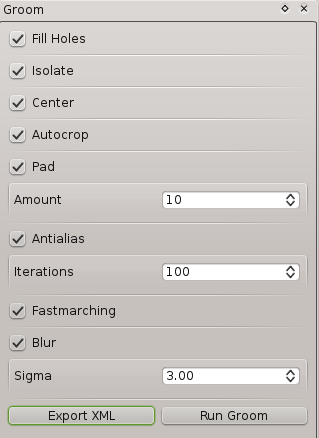
\includegraphics[width=0.4\textwidth]{figs/supershapes_groom.png}
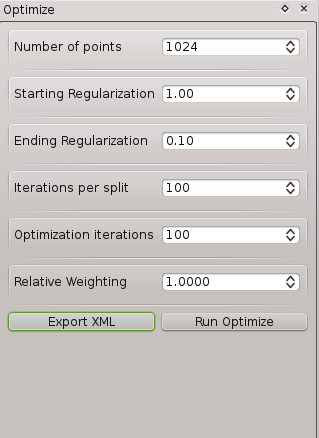
\includegraphics[width=0.4\textwidth]{figs/supershapes_optimize.png}
\caption{Groom and optimize parameters for supershape datasets }
\label{fig:supershape_params}
\end{figure}

\vspace{0.1in}
\begin{figure}[!htp]
\centering
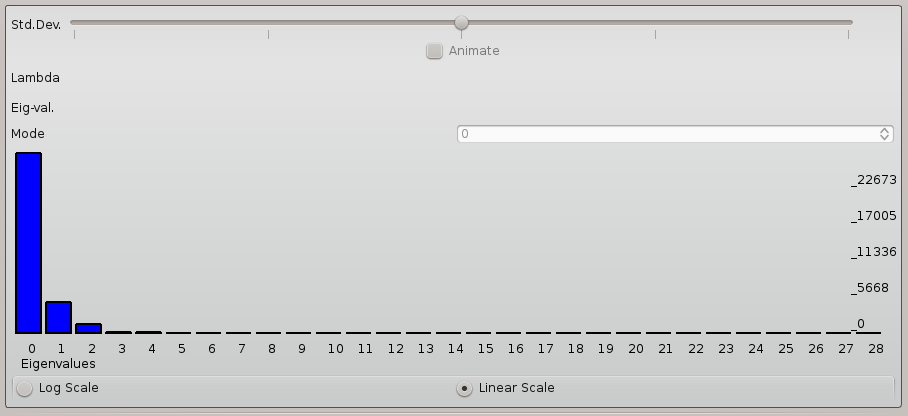
\includegraphics[width=0.7\textwidth]{figs/supershapes_1mode_spectrum.png}\vspace{0.1in}\\
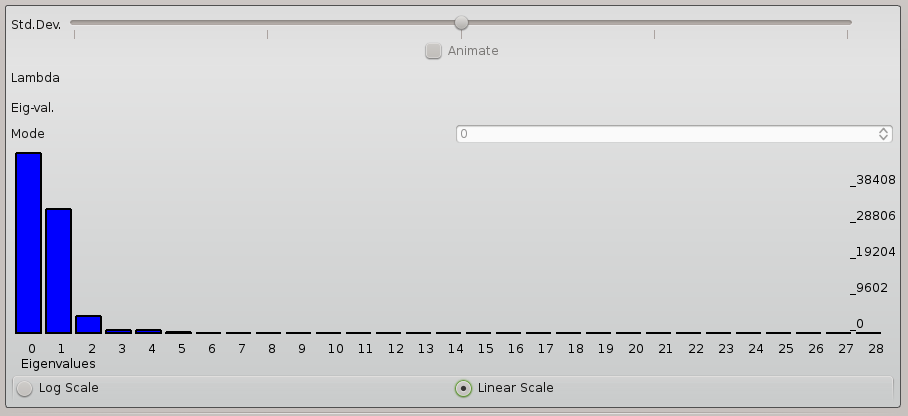
\includegraphics[width=0.7\textwidth]{figs/supershapes_2mode_spectrum.png}\vspace{0.1in}\\
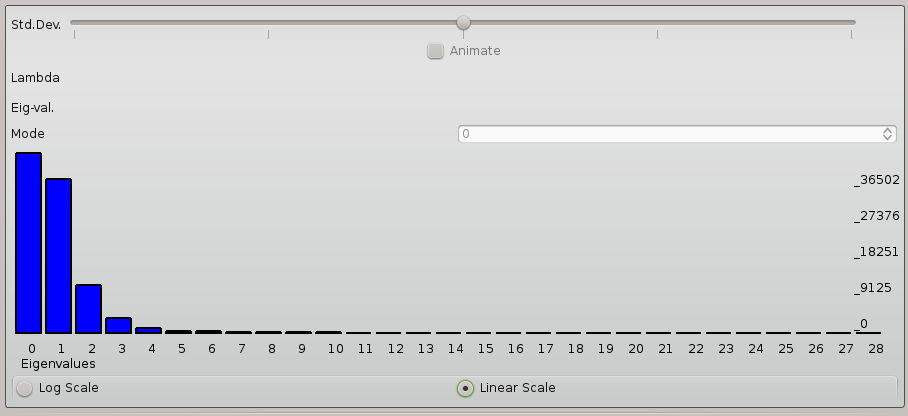
\includegraphics[width=0.7\textwidth]{figs/supershapes_3mode_spectrum.png}
\caption{Eigen spectrum of supershape datasets. Top: \texttt{supershape3\char`_1modes}. Middle: \texttt{supershape3\char`_2modes}. Bottom: \texttt{supershape3\char`_3modes} }
\label{fig:supershape_spectrums}
\end{figure}

\vspace{0.1in}
\begin{figure}[!htp]
\centering
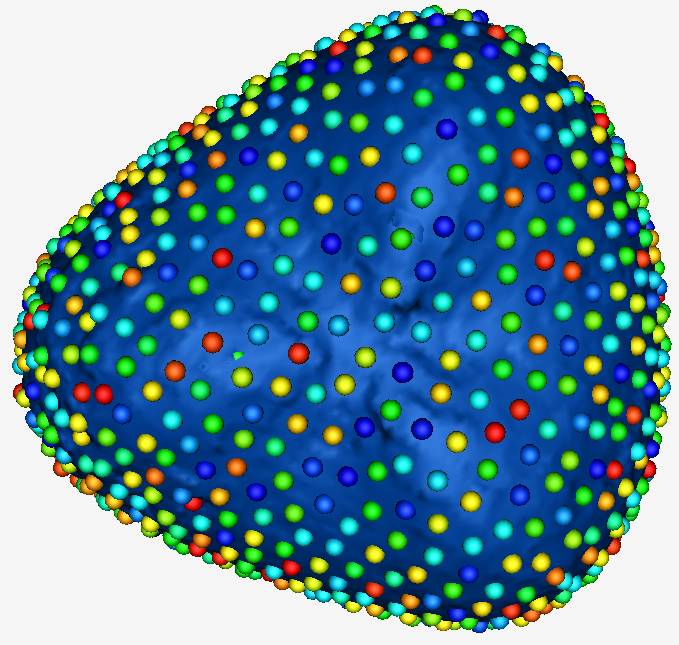
\includegraphics[width=0.3\textwidth]{figs/supershapes_3mode_mod1_neg1std.png}
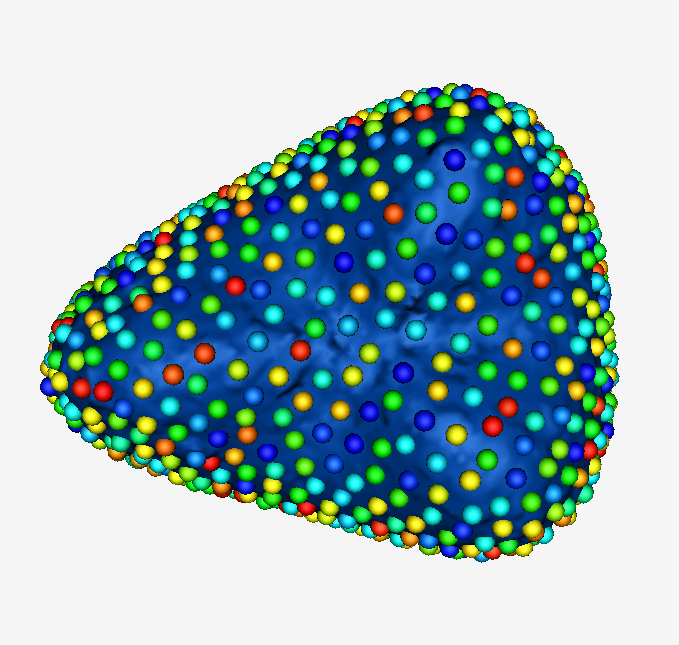
\includegraphics[width=0.3\textwidth]{figs/supershapes_3mode_mod1_0std.png}
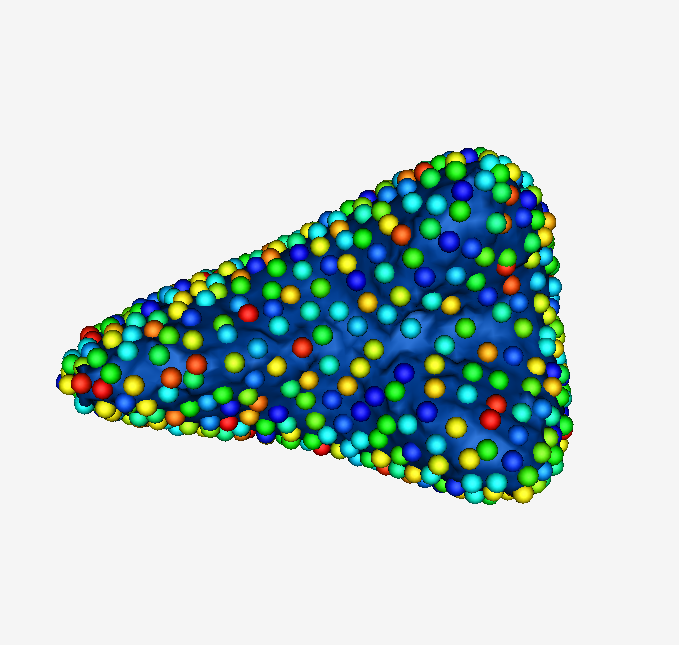
\includegraphics[width=0.3\textwidth]{figs/supershapes_3mode_mod1_1std.png}
\caption{The variation of \texttt{supershape3\char`_3modes} along the first mode. Left: $\mu - 1\sigma$. Middle: $\mu$. Right: $\mu + 1\sigma$. Note the first mode captures the scale in the y-direction}
\label{fig:supershape_3modes_mod1}
\end{figure}

\vspace{0.1in}
\begin{figure}[!htp]
\centering
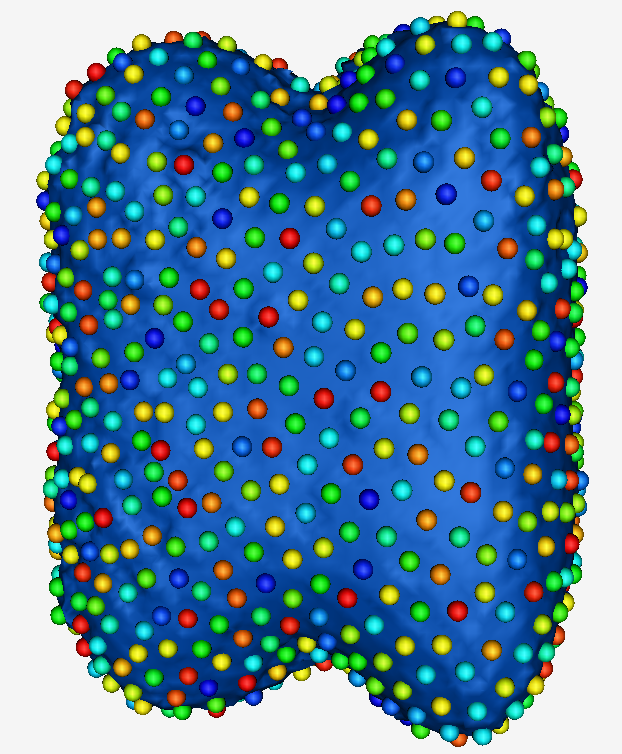
\includegraphics[width=0.3\textwidth]{figs/supershapes_3mode_mod2_neg1std.png}
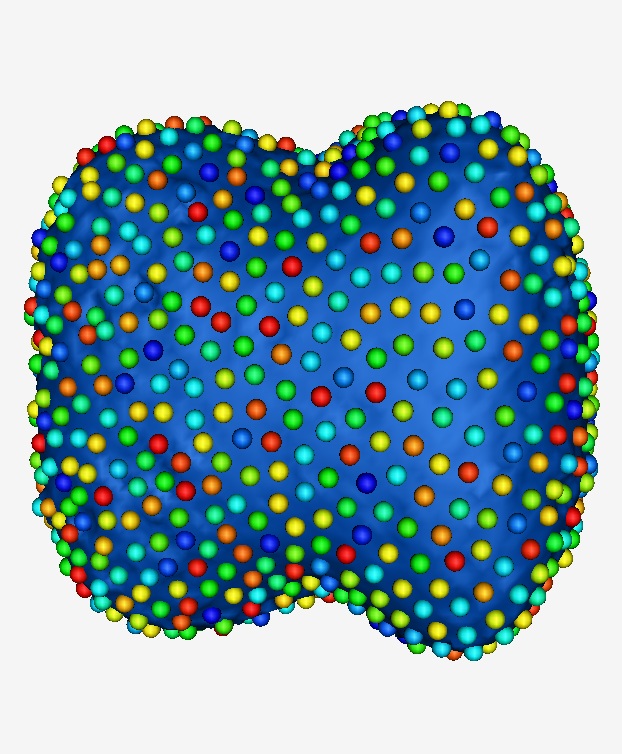
\includegraphics[width=0.3\textwidth]{figs/supershapes_3mode_mod2_0std.png}
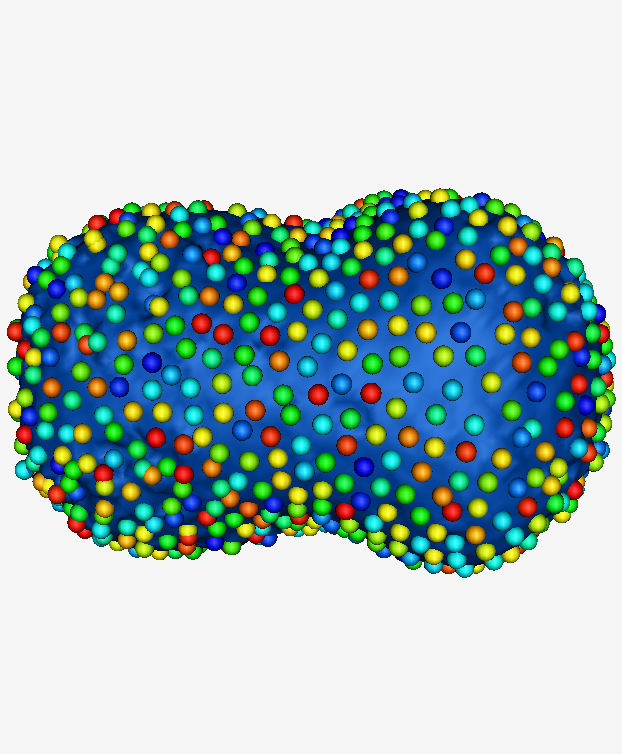
\includegraphics[width=0.3\textwidth]{figs/supershapes_3mode_mod2_1std.png}
\caption{The variation of \texttt{supershape3\char`_3modes} along the second mode. Left: $\mu - 1\sigma$. Middle: $\mu$. Right: $\mu + 1\sigma$. Note the second mode captures the scale in the z-direction}
\label{fig:supershape_3modes_mod2}
\end{figure}

\vspace{0.1in}
\begin{figure}[!htp]
\centering
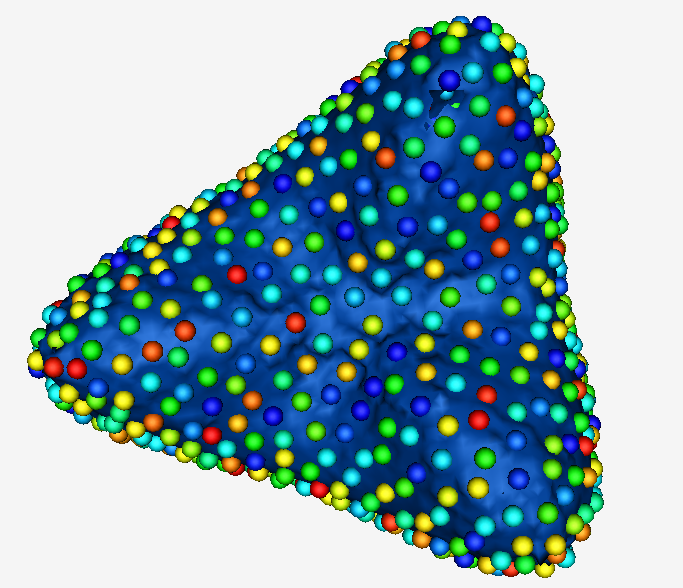
\includegraphics[width=0.3\textwidth]{figs/supershapes_3mode_mod3_neg1std.png}
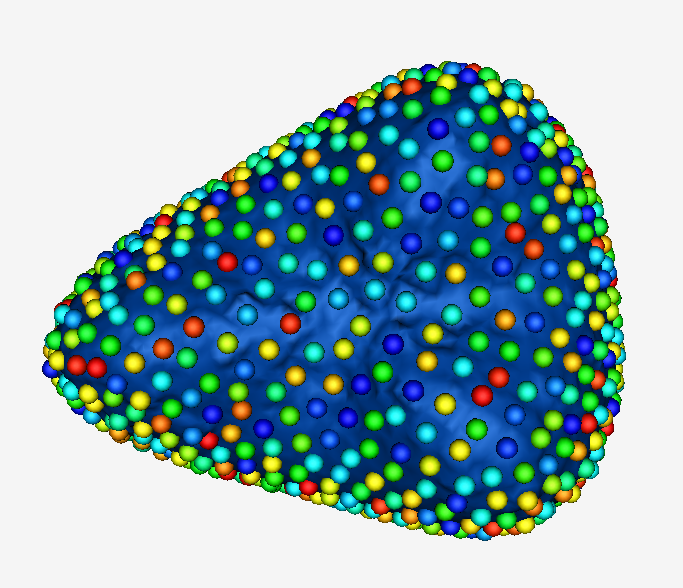
\includegraphics[width=0.3\textwidth]{figs/supershapes_3mode_mod3_0std.png}
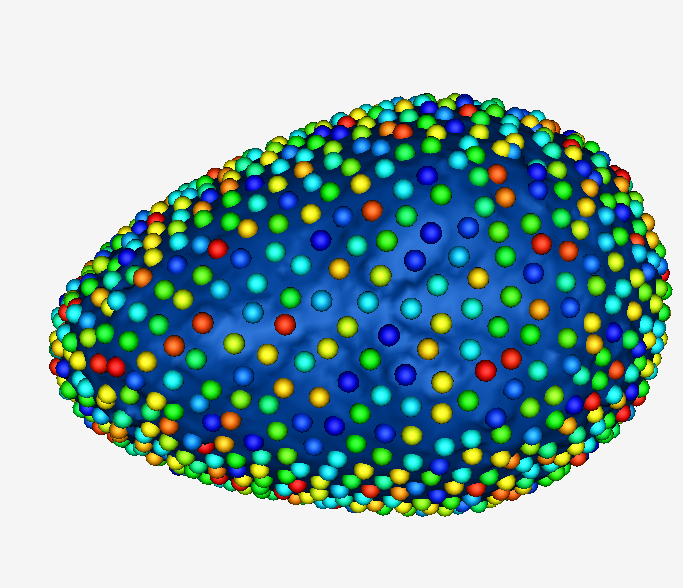
\includegraphics[width=0.3\textwidth]{figs/supershapes_3mode_mod3_1std.png}
\caption{The variation of \texttt{supershape3\char`_3modes} along the third mode. Left: $\mu - 1\sigma$. Middle: $\mu$. Right: $\mu + 1\sigma$. Note the third mode captures shape variation according to the $(n_2, n_3)$ supershape parameters}
\label{fig:supershape_3modes_mod3}
\end{figure}


\section{Contact and Bug Reports}

Please email any questions to \texttt{shapeworks-users@sci.utah.edu}. If there problems or bugs, please report them using the issue tracker on GitHub \texttt{https://github.com/SCIInstitute/ShapeWorksStudio/issues}. This includes feature requests. Feel free to add improvements using git pull requests. 

%\bibliographystyle{osajnl} 
%\bibliography{references.bib}
\end{document}
